\documentclass[11pt]{report}

\usepackage{geometry} % See geometry.pdf to learn the layout options. There are lots.
\geometry{a4paper} %or letterpaper or a5paper or ... 

%for figures and graphics
\usepackage{graphicx}
\DeclareGraphicsRule{.tif}{png}{.png}{`convert #1 `dirname #1`/`basename #1 .tif`.png}

%\input imports all commands from the target files
%The idea behind this file is that it will be used to store all the maths-related macros that I concoct; so that I can import all the commands by \input{this file} in the preamble of any file that I want to use them in.
%This should make the top-level files look a lot cleaner, and the preamble much shorter!

\usepackage{amssymb}
\usepackage{amsmath}

%theorems and lemma etc setup using amsthm
\usepackage{amsthm}
\newcommand{\tstk}[1]{\textbf{#1} \newline}
\theoremstyle{definition}
\newtheorem{definition}{Definition}[section]
\theoremstyle{plain}
\newtheorem{theorem}{Theorem}[section]
\theoremstyle{plain}
\newtheorem{lemma}[theorem]{Lemma}
\theoremstyle{plain}
\newtheorem{prop}[theorem]{Proposition}

\allowdisplaybreaks %allows equations in the same align environment to split over multiple pages.

%begin the macros via newcommand. Try to group them up reasonably!

%standard sets
\newcommand{\naturals}{\mathbb{N}}			%natural numbers
\newcommand{\integers}{\mathbb{Z}}			%integers
\newcommand{\rationals}{\mathbb{Q}}			%rational numbers
\newcommand{\reals}{\mathbb{R}}				%real numbers
\newcommand{\complex}{\mathbb{C}}			%complex numbers

%brackets and norms
\newcommand{\bracs}[1]{\left( #1 \right)}				%encloses input in brackets
\newcommand{\sqbracs}[1]{\left[ #1 \right]}				%encloses input in square brackets
\newcommand{\clbracs}[1]{\left\{ #1 \right\}}			%encloses input in curly bracers
\newcommand{\abs}[1]{\lvert #1 \rvert}					%absolute value
\newcommand{\norm}[2]{\lvert\lvert #1 \rvert\rvert}		%norm (double line)

%function sets
\newcommand{\smooth}[1]{C^{\infty}\bracs{#1}}							%smooth functions
\newcommand{\ltwo}[2]{L^{2}\bracs{#1,\mathrm{d}#2}}						%general L^2 space
\newcommand{\gradSob}[2]{H^1_\mathrm{grad}\bracs{#1, \mathrm{d}#2}}		%gradient Sobolev space
\newcommand{\curlSob}[2]{H^1_\mathrm{curl}\bracs{#1, \mathrm{d}#2}}		%curl Sobolev space
\newcommand{\kSob}[2]{H^1_{k,\mathrm{curl}}\bracs{#1, \mathrm{d}#2}}	%k-curl Sobolev space

%grad and curl sets
\newcommand{\gradZero}[2]{\mathcal{G}_{ #1, \mathrm{d}#2}\bracs{0}}		%gradients of zero for domain #1 with measure #2
\newcommand{\curlZero}[2]{\mathcal{C}_{ #1, \mathrm{d}#2}\bracs{0}}	%curls of zero for domain #1 with measure #2

%derivatives and grad-like symbols
\newcommand{\diff}[2]{\dfrac{\mathrm{d}#1}{\mathrm{d}#2}}			%complete derivative d#1/d#2
\newcommand{\pdiff}[2]{\dfrac{\partial #1}{\partial #2}}			%partial derivative p#1/p#2
\newcommand{\ddiff}[2]{\dfrac{\mathrm{d}^2 #1}{\mathrm{d}^2 #2}}	%2nd deriv
\newcommand{\grad}{\nabla}											%grad operator
\newcommand{\curl}[1]{\grad_{#1}\wedge}								%curl with measure subscript #1

%displaying integrals
\newcommand{\integral}[3]{\int_{#1}#2 \ \mathrm{d}#3}			%integral, domain #1, integrand #2, measure #3

%notation for variable use throughout the file
\newcommand{\dddom}{\widetilde{\Omega}}			%3D domain notation
\newcommand{\ddom}{\Omega}						%2D domain notation
\newcommand{\dddmes}{\widetilde{\mu}}			%3D measure
\newcommand{\ddmes}{\mu}						%2D measure

\newcommand{\graph}{\mathbb{G}}					%graph variable %maths commands, variables, and other packages
\usepackage{tikz}

%tikz structures and patterns
\usetikzlibrary{patterns}

%this defines a fill pattern called hexagons
\def\hexagonsize{0.2cm}
\pgfdeclarepatternformonly
  {hexagons}% name
  {\pgfpointorigin}% lower left
  {\pgfpoint{3*\hexagonsize}{0.866025*2*\hexagonsize}}%  upper right
  {\pgfpoint{3*\hexagonsize}{0.866025*2*\hexagonsize}}%  tile size
  {% shape description
   \pgfsetlinewidth{1.2pt}
   \pgftransformshift{\pgfpoint{0mm}{0.866025*\hexagonsize}}
   \pgfpathmoveto{\pgfpoint{0mm}{0mm}}
   \pgfpathlineto{\pgfpoint{0.5*\hexagonsize}{0mm}}
   \pgfpathlineto{\pgfpoint{\hexagonsize}{-0.866025*\hexagonsize}}
   \pgfpathlineto{\pgfpoint{2*\hexagonsize}{-0.866025*\hexagonsize}}
   \pgfpathlineto{\pgfpoint{2.5*\hexagonsize}{0mm}}
   \pgfpathlineto{\pgfpoint{3*\hexagonsize+0.2mm}{0mm}}
   \pgfpathmoveto{\pgfpoint{0.5*\hexagonsize}{0mm}}
   \pgfpathlineto{\pgfpoint{\hexagonsize}{0.866025*\hexagonsize}}
   \pgfpathlineto{\pgfpoint{2*\hexagonsize}{0.866025*\hexagonsize}}
   \pgfpathlineto{\pgfpoint{2.5*\hexagonsize}{0mm}}
   \pgfusepath{stroke}
  } 

\newcommand{\Tube}[6][]%
% [further options], width, iterations, inner color, outer color, path definition
{   \colorlet{InColor}{#4}
    \colorlet{OutColor}{#5}
    \foreach \I in {1,...,#3}
    {   \pgfmathsetlengthmacro{\h}{(\I-1)/#3*#2}
        \pgfmathsetlengthmacro{\r}{sqrt(pow(#2,2)-pow(\h,2))}
        \pgfmathsetmacro{\c}{(\I-0.5)/#3*100}
        \draw[InColor!\c!OutColor, line width=\r, #1] #6;
    } 
} %draws a 3D-tube, see https://tex.stackexchange.com/questions/148379/define-a-path-like-command-in-tikz-to-draw-3d-tubes for details
 %tikz things, including importing tikz itself

%labelling hacks
\newcommand\labelthis{\addtocounter{equation}{1}\tag{\theequation}}

%reminders of things to fill in
%\newcommand{\tstk}[1]{\textbf{#1}\newline}

\title{All Work and Results}  % Declares the document's title.
\author{Will Graham (W.Graham@bath.ac.uk) \cite{graham2018citation}}      % Declares the author's name.
\date{\today}      % commenting out this command produces today's date.

%-------------------------------------------------------------------------
%DOCUMENT STARTS

\begin{document}

%TITLE AND CONTENTS ETC; comment out to save computing time

%\maketitle 					%create title
%\tableofcontents 			%have a contents page
%\newpage 					%begin the actual report on a new page

%REPORT BEGINS

%\input chapters one at a time; the references should all match up and can even cross-reference; however you won't get prompts for references across files when editing.
%NB: Can use \include for speed, but then the directory fills up with useless .aux files.
%To save time, comment out sections that aren't being edited. References may disappear but the file will still compile!

%\chapter{Introduction} \label{ch:1Intro}

\section{Motivation}
Optical fibres are the \textit{de facto} industry standard for large telecommunications systems, thanks to their ability to transmit information quickly and with far less signal loss than other methods (such as metal cables).
The technology has rapidly developed since the first optical fibres were fabricated in the 1970s \cite{knight2003photonic} and optical fibres in use today present a balance between several competing factors to deliver a reliable performance.
Factors such as (optical) loss are inherent, brought about by the materials needed to build the fibres; whilst other factors can be influenced by design (group-velocity dispersion) or the fabrication process (which can lead to imperfections and polarisation effects).
Despite the technological developments of the fibres, the underpinning physical processes remain unchanged --- all improvements to the technology have been incremental and largely centre around the manufacturing process.
The fibre will have a core made of a dielectric (non-conducting) material with a given refractive index and will be surrounded by a cladding; another dielectric material of a lower refractive index.
Typically the difference in refractive indices of the core and cladding is very small \tstk{silica fibres and doping, get some numbers}. 
By choosing a lower refractive index for the cladding material than the core, modes of light\footnote{A mode of light is a mono-frequency solution to the governing equations of electromagnetism in the fibre.} can be confined to the core of an optical fibre via the phenomenon of Total Internal Reflection (TIR) \tstk{reference, cba to explain as it's not important to the report}, allowing guided propagation of light over \tstk{actual distance?} hundreds of kilometres.\newline

Photonic crystal fibres (PCFs) are a departure from the setup of core surrounded by cladding \cite{russell2003photonic}; instead relying on the micro-structure of the photonic crystal to alter the optical properties of the fibre it forms.
This microstructure can cause the crystal to exhibit band-gaps; frequency ranges where there are no propagating modes of light in the crystal, despite the existence of propagating modes at lower (and/or higher) frequencies.
These band-gaps allow for light to be confined to core materials previously thought impossible (like air), or even when the core itself consists of vacuum.
This gives rise to the idea of a ``hollow-core fibre"; a PCF with air (or vacuum) as its core material, guiding light at frequencies determined by the band-gaps of the photonic crystal itself.
For the record, PCFs can also be ``solid core", that is have a more conventional material like silica as the core material, or even have metallic cores \tstk{David's paper he gave us}.
Crucially though, PCFs do not use TIR to guide light but rather exploit the fact that light at particular frequencies is confined to the cores simply because it is unable to propagate in the surrounding crystal, due to the optical properties bestowed on the crystal by its micro-structure.
\tstk{illustrative diagram of fibre differences?}

\section{Background}
In physical applications the 2D cross section is often composed of one or more material inclusions, which can give rise to interesting phenomena in the resulting wave propagation problems (such as band-gap spectra).
These inclusions themselves are often arranged in a periodic structure (where applicable), and the model that one considers for a waveguide will inevitably depend on how one chooses to treat these inclusions.
For our approach we shall define a ``waveguide surface" on which to pose our wave propagation problem, and appropriate boundary conditions at the inclusion interfaces.
Such a problem can be arrived at from appropriate treatment of ``high-contrast" media problems; which reduce a problem on a domain with inclusions to a problem on the inclusions with altered boundary data, representing the information from the original problem.
However in the approach we shall be taking, we will look to formulate our model from a measure-theoretic perspective, which will allow us to retain a level of generality surrounding the geometry we choose to impose on our waveguide. 
In the domains with periodic structure in the $\bracs{x_1,x_2}$-plane, we will often assume this periodic structure to extend infinitely and possess a finite period cell, rather than a periodic pattern extending over a finite region of space.
This is because tools such as the Gelfand transform allow us to reduce a problem on an infinite periodic structure to a family of problems on the period cell which parametrised by the so-called quasi-momentum, which we will elaborate on later.
\tstk{this is more about making sure we have some meaning behind being on the spectrum of operators, so might be better kept for that section}
\tstk{literature review, both David's papers on existing modelling techniques and fibre specs, plus from the analysis side (Zhikov etc).}

\section{Setup} \label{sec:Setup}
We wish to study wave propagation problems on waveguide-like structures in a variety of physical contexts, including \tstk{the aforementioned?}
\begin{itemize}
	\item Electromagnetism (photonic crystal fibres),
	\item Elasticity,
	\item Piezo-elasticity.
\end{itemize}
To this end, we shall consider domains of the form $\dddom = \ddom\times I$ where $I\subset\reals$.
The domain $\dddom$ represents the space the waveguide occupies; $\ddom$ represents the 2-dimensional cross-section of the waveguide in the $\bracs{x_1,x_2}$-plane, which is translation invariant along the axis of the waveguide in the $x_3$ direction.
An illustration of this is provided in figure \ref{fig:IntroStrucDiagram}.
\begin{figure}[h!]
	\centering
	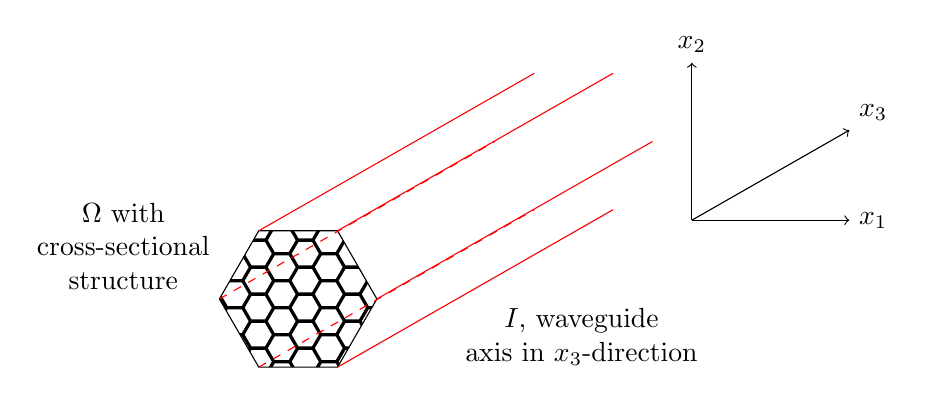
\begin{tikzpicture}
		%2d plane $\ddom$
		\filldraw[pattern=hexagons] (0.5,0.866025) -- (1,0) -- (0.5,-0.866025) -- (-0.5,-0.866025) -- (-1,0) -- (-0.5,0.866025) -- cycle;
		\node[anchor=south east, align=center] at (-1,0) {$\ddom$ with \\ cross-sectional \\ structure};
		
		%1d extension as fibre/waveguide
		\draw[red] (-0.5,0.866025) -- (3, 2.866025);		
		\draw[red] (0.5,0.866025) -- (4, 2.866025);
		\draw[red] (1,0) -- (4.5, 2);
		\draw[red] (0.5,-0.866025) -- (4,2-0.866025);
		\draw[dashed, red] (-0.5,-0.866025) -- (3,2-0.866025);
		\draw[dashed, red] (-1,0) -- (2.5,2);
		\node[anchor=north west, align=center] at (2,0) {$I$, waveguide \\ axis in $x_3$-direction};
		
		%axes labels
		\draw[->] (5,1) -- (7,1) node[anchor=west] {$x_1$};
		\draw[->] (5,1) -- (5,3) node[anchor=south] {$x_2$};
		\draw[->] (5,1) -- (7,1+8/7) node[anchor=south west] {$x_3$};
	\end{tikzpicture}
	\caption{\label{fig:IntroStrucDiagram} Illustration of the waveguide domains that we shall be considering. The domains consist of cross-sectional structure in the $\bracs{x_1,x_2}$-plane which is translation invariant in $x_3$, the direction down the waveguide. The specifics of the structure in the $\bracs{x_1,x_2}$-plane depend on the waveguide we wish to model.}
\end{figure}
The choice of $I$ dictates how we choose to treat the structure we are modelling mathematically; $I=[0,\infty)$ represents a waveguide with an ``entrance" or ``beginning", the choice of $I=\reals$ in the $x_3$-direction represents an ``infinitely long waveguide", and the choice of $I$ being a finite interval represents a waveguide linking two locations. \newline


\chapter{Scalar Equations} \label{ch:ScalarEqns}
In this chapter we look at scalar wave equations in our waveguide-like geometry, treating the cross-sectional structure as singular.
We base our approach largely off the work of Zhikov \cite{zhikov2000extension}, in that we consider what can be colloquially described as ``differential equations with respect to a measure $\ddmes$".
We will give a rigorous definition of the kinds of problems and spaces that this colloquialism covers in the following sections, and will demonstrate how this framework allows us to obtain a quantum graph problem from our variational formulation.
This will allow us to make use of the theory which was highlighted in \ref{ch:QuantumGraphs}, and additionally will make our variational problems open to numerical solution.
At the conclusion of this chapter we will have highlighted the techniques that are available to us, and how we shall adapt them for the more descriptive (or physical) vector systems we consider in chapter \ref{ch:VectorEqns}.

\section{The Scalar Sobolev Spaces} \label{sec:ScalarSobSpaces}
In this section we look to construct the function spaces that we shall be working with throughout the chapter, as well as discussing some of the consequences of this construction.
What we present is a synopsis of the work of Zhikov presented in \cite{zhikov2000extension}, although with an adapted notation which will suit our needs when we later make a link to Quantum Graph problems. \newline

Let $N\in\naturals$, $D\subset\reals^N$ and $\nu$ be a (Borel) measure on $D$.
Denote the set of smooth functions on $D$ by $\smooth{D}$, and then let $W=W\bracs{D,\mathrm{d}\nu}$ be the closure of the set of pairs $\bracs{\phi,\grad\phi}$ in $\ltwo{D}{\nu}\times\ltwo{D}{\nu}^N$, where $\phi\in\smooth{D}$.
That is
\begin{align*}
	W = W\bracs{D,\nu} &= \overline{\clbracs{\bracs{\phi,\grad\phi} \ \vert \ \phi\in\smooth{D}}} \quad \text{in} \ \ltwo{D}{\nu}\times\ltwo{D}{\nu}^N.
\end{align*}
The notation above is chosen to provide similarities to the $W$-style construction of classical Sobolev spaces (in which integration is performed with respect to the $N$-dimensional Lebesgue measure).
An element of $W$ is a pair $\bracs{u,z}$; and as the above construction suggests we would like to associate the function $z$ with a distributional derivative of sorts, however there is a problem with making this association.
Suppose that $\bracs{u,z}\in W$ and $\bracs{0,y}\in W$, then we also have $\bracs{u,z+y}\in W$ too by taking an approximating sequence for each pair and forming another sequence by point-wise addition of terms.
As a result each $u\in\ltwo{D}{\nu}$ has multiple (distinct) functions $z\in\ltwo{D}{\nu}^n$ such that $\bracs{u,z}\in W$; and so as it stands it does not make sense to associate ``\textit{a} gradient" to $u$, because $u$ has multiple candidates for this role.
In what follows we will look into this quirk, and deduce that we can make sense of the idea of ``\textit{the} gradient". \newline

Let use denote the set of ``gradients of zero" by $\gradZero{D}{\nu}$, that is
\begin{align*}
	\gradZero{D}{\nu} &= \clbracs{z\in\ltwo{D}{\nu}^N \ \vert \ \bracs{0,z}\in W}, \\
	&= \clbracs{z\in\ltwo{D}{\nu}^N \ \vert \ \exists\phi_n\in\smooth{D} \text{ such that } \phi_n\lconv{\ltwo{D}{\nu}}0, \grad\phi_n\lconv{\ltwo{D}{\nu}^N}z}, \labelthis\label{eq:GradZeroSequenceDefinition}
\end{align*}
the construction of $W$ ensuring the two sets coincide.
A fact that follows immediately from this definition and will be used later is that $\gradZero{D}{\nu}$ is a closed linear subspace of $\ltwo{D}{\nu}^N$.
The illustration of the non-uniqueness of gradients earlier employed the fact that we can always add an element of $\gradZero{D}{\nu}$ to the second member of a pair $\bracs{u,z}\in W$ and produce another element of $W$.
Colloquially this can be expressed by the following statement; we can always ``add a gradient of zero" to an existing ``gradient", which will produce another ``gradient".
This hints at the possibility that whilst we any $u$ may not have a unique gradient, it might at least have only one relevant gradient in the context of a mathematical problem.
With this in mind, consider the following variational problem; find a pair $\bracs{u,z}\in W$ such that
\begin{align} \label{eq:TangentialGradientVariationalMotivation}
	\integral{D}{z \cdot \grad\overline{\phi} - u\overline{\phi}}{\nu} &= 0 \quad \forall\phi\in\smooth{D}.
\end{align}
Setting aside questions of existence and uniqueness of solutions to this problem for the purposes of illustration, take an element $g\in\gradZero{D}{\nu}$, and an approximating sequence $\phi_n$ as in the definition \eqref{eq:GradZeroSequenceDefinition}.
Substituting $\phi_n$ into \eqref{eq:TangentialGradientVariationalMotivation} and employing a limit-argument, we can see that
\begin{align*}
	\integral{D}{z \cdot g}{\nu} &= 0 \quad \forall g\in\gradZero{D}{\nu}.
\end{align*}
Namely that the member $z$ of the solution pair is orthogonal (in the $\ltwo{D}{\nu}$-norm) to $\gradZero{D}{\nu}$.
Stepping back for a moment, as $\gradZero{D}{\nu}$ is a closed linear subspace of $\ltwo{D}{\nu}^N$ we can decompose $\ltwo{D}{\nu}^N$ as
\begin{align*}
	\ltwo{D}{\nu}^N &= \gradZero{D}{\nu}^{\perp} \oplus \gradZero{D}{\nu}.
\end{align*}
But we have just seen that the member of the solution pair $z\in\gradZero{D}{\nu}^{\perp}$, hence $z$ is the \textit{unique} element of $\gradZero{D}{\nu}^{\perp}$ such that every pair $\bracs{u,\tilde{z}}\in W$ can be written as $\bracs{u,z+g}\in W$ for some $g\in\gradZero{D}{\nu}$.
Thus whilst the concept of a unique gradient does not make sense in this setting, once we consider variational problems we can obtain the concept of the \textit{tangential} gradient $z$, which is unique.
We therefore adopt the notation $z := \grad_\nu u$ for the second member of the solution pair $\bracs{u,z}\in W$, and can now define the (non-classical) ``Sobolev space"
\begin{align*}
	\gradSob{D}{\nu} &:= \clbracs{\bracs{u,\grad_\nu u}\in W \ \vert \ \grad_\nu u \perp \gradZero{D}{\nu}}.
\end{align*}
Furthermore we can now pose variational problems on this space; for example we would write \eqref{eq:TangentialGradientVariationalMotivation} as find $\bracs{u,\grad_\nu u}\in\gradSob{D}{\nu}$ such that
\begin{align} \label{eq:GeneralVariationProblem}
	\integral{D}{\grad_\nu u \cdot \grad\overline{\phi} - u\overline{\phi}}{\nu} &= 0 \quad \forall\phi\in\smooth{D}.
\end{align}
As $\grad_\nu u$ is unique for each $u$ it is sufficient to specify only the element $u$ to identify the pair $\bracs{u,\grad_\nu u}\in\gradSob{D}{\nu}$, so henceforth we adopt the shorthand $u\in\gradSob{D}{\nu}$ to refer to this element.
We also adopt a shorthand notation for the problem \eqref{eq:GeneralVariationProblem}, writing is as
\begin{align} \label{eq:GeneralDifferentialProblem}
	-\grad_\nu^2 u + u &= 0, \quad u\in\gradSob{D}{\nu}.
\end{align}
Of course this is just notation and has no meaning without \eqref{eq:GeneralVariationProblem}; one can envisage \eqref{eq:GeneralDifferentialProblem} as somehow being the weak form of \eqref{eq:GeneralVariationProblem} for analogy with classical Sobolev spaces and variational problems, however there is not formal link in this context (mainly because of the lack of the ``integration by parts" technique). \newline

In general for $f\in\ltwo{D}{\nu}$ and an elliptic matrix $A(x)$, we say that $u\in\gradSob{D}{\nu}$ is a solution to the (elliptic) equation
\begin{align} \label{eq:GeneralScalarStrongForm}
	-\grad_\nu \cdot \bracs{A(x)\grad_\nu u(x)} &= f(x), \quad x\in D
\end{align}
to mean that $u\in\gradSob{D}{\nu}$ solves the variational problem
\begin{align} \label{eq:GeneralScalarWeakForm}
	\integral{D}{A\grad_\nu u \cdot \grad\overline{\phi}}{\nu} &= \integral{D}{f\overline{\phi}}{\nu} \quad \forall \phi\in\smooth{D}.
\end{align}
Again it is critical to highlight that \eqref{eq:GeneralScalarWeakForm} is the only way for us to assign a meaning to the problem \eqref{eq:GeneralScalarStrongForm}.
However existence and uniqueness of the solution pair $\bracs{u,\grad_\nu u}$ is guaranteed by appealing to the Riesz Representation theorem and the bilinear form defined by \eqref{eq:GeneralScalarWeakForm}.
One can (see \cite{zhikov2000extension}) establish that the $\grad_\nu u$ in the solution pair coincides with the unique gradient of $u$ such that $A\grad_\nu u \perp \gradZero{D}{\nu}$; highlighting that understanding $\gradZero{D}{\nu}$ is crucial to determining solutions to \eqref{eq:GeneralScalarStrongForm}.
For completeness, we also note that the spectral problem (when $f$ is replaced by $\lambda u$ for some eigenvalue $\lambda\in\complex$) is written as
\begin{align*}
	-\grad_\nu \cdot \bracs{A(x)\grad_\nu u(x)} &= \lambda u(x), \quad x\in D
\end{align*}
to mean
\begin{align*}
	\integral{D}{A\grad_\nu u \cdot \grad\overline{\phi}}{\nu} &= \lambda\integral{D}{u\overline{\phi}}{\nu} \quad \forall \phi\in\smooth{D}.
\end{align*}
In which case solutions (if they exist) are triplets $\bracs{\lambda, u, \grad_\nu u}$, although it suffices to specify $\bracs{\lambda, u}$ only. \newline

To conclude this section we present some general results that we will need later in our analysis.
The first is a simple result which makes proving membership of $\gradSob{D}{\nu}$ easier, and is presented in \cite{zhikov2002homogenization} as lemma 5.5.
\begin{prop}[Sufficient Condition for Membership of $\gradSob{D}{\nu}$] \label{prop:Lemma5-5}
	Suppose we have a sequence $u_n\in\gradSob{D}{\nu}$ such that $u_n\rightarrow u$ in $\ltwo{D}{\nu}$ for some $u\in\ltwo{D}{\nu}$, and that the sequence of tangential gradients $\grad_\nu u_n$ is bounded in $\ltwo{D}{\nu}^N$.
	Then 
	\begin{align*}
		u\in\gradSob{D}{\nu};
	\end{align*}
	that is, $\grad_\nu u$ exists and the pair $\bracs{u,\grad_nu u}\in\gradSob{D}{\nu}$).
\end{prop}
\begin{proof}
	As $\grad_\nu u_n$ is bounded in $\ltwo{D}{\nu}^N$ it has a convergent subsequence that we denote by $\grad_\nu u_{n_k}$, and this sequence has some limit $v\in\ltwo{D}{\nu}^N$.
	Note that since $\grad_\nu u_{n_k}\in\gradZero{D}{\nu}^\perp$ for all $k\in\naturals$, the limit $v\in\gradZero{D}{\nu}^\perp$ too.
	Furthermore the corresponding subsequence $u_{n_k}$ of $u_n$ still converges in $\ltwo{D}{\nu}$ to $u$, being a subsequence of a convergent sequence.
	Now for each $k\in\naturals$ there exists an sequence of smooth functions $\phi_{k,l}$ such that
	\begin{align*}
		\phi_{k,l}\lconv{\ltwo{D}{\nu}} u_{n_k}, &\quad \grad\phi_{k,l}\lconv{\ltwo{D}{\nu}^n}\grad u_{n_k}, \toInfty{l}.
	\end{align*}
	We can therefore apply a diagonal argument to find a sequence of smooth functions $\phi_{k, l_k}$ such that
	\begin{align*}
		\phi_{k,l_k}\lconv{\ltwo{D}{\nu}} u, &\quad \grad\phi_{k,l_k}\lconv{\ltwo{D}{\nu}^N}v, \toInfty{k}.
	\end{align*}
	Since $v\in\gradZero{D}{\nu}^\perp$, we conclude that $v = \grad_\nu u$ and thus
	\begin{align*}
		\bracs{u, \grad_\nu u}\in \gradSob{D}{\nu}.
	\end{align*}
\end{proof}

The second result that we present is essentially the equivalent of the product rule for tangential gradients.
\begin{prop}[Product Rule for Tangential Gradients] \label{prop:ProductRuleGradients}
	Suppose $u,v\in\gradSob{D}{\nu}$.
	Then we also have that
	\begin{align*}
		\bracs{uv, u\grad_\nu v + v\grad_\nu u}\in\gradSob{D}{\nu}.
	\end{align*}
\end{prop}
\begin{proof}
	Take smooth sequences $\phi_l, \psi_l$ such that
	\begin{align*}
		\phi_l \lconv{\ltwo{D}{\nu}} u, &\quad \grad\phi_l \lconv{\ltwo{D}{\nu}^N} \grad_\nu u, \\
		\psi_l \lconv{\ltwo{D}{\nu}} v, &\quad \grad\psi_l \lconv{\ltwo{D}{\nu}^N} \grad_\nu v.
	\end{align*}
	Note that because of these convergences, the sequences 
	\begin{align*}
		\norm{\phi_l}_{\ltwo{D}{\nu}}, \norm{\psi_l}_{\ltwo{D}{\nu}}, \norm{\grad\phi_l}_{\ltwo{D}{\nu}^N}, \norm{\grad\psi_l}_{\ltwo{D}{\nu}^N}.
	\end{align*}
	are all bounded in $\reals$.
	We now examine the sequence formed from term-wise products, $\phi_l\psi_l$.
	Note that this remains a sequence of smooth functions, and we have that $\phi_l\psi_l \rightarrow uv \toInfty{l}$ by the Algebra of Limits in $\ltwo{D}{\nu}$.
	Furthermore,
	\begin{align*}
		\recip{4}\integral{D}{\abs{ \grad\bracs{\phi_l\psi_l} - u\grad_\nu v - v\grad_\nu u }^2}{\nu}
		&\leq \recip{2}\integral{D}{\abs{ \phi_l\grad\psi_l - u\grad_\nu v }^2}{\nu} \\
		& \ + \recip{2}\integral{D}{\abs{ \psi_l\grad\phi_l - v\grad_\nu u }^2}{\nu} \\
		&\leq \norm{\phi_l - u}_{\ltwo{D}{\nu}}^2\norm{\grad\psi_l}_{\ltwo{D}{\nu}^N}^2 \\
		& \ + \norm{u}_{\ltwo{D}{\nu}}^2\norm{\grad\psi_l - \grad_\nu v}_{\ltwo{D}{\nu}^N}^2 \\
		& \ + \norm{\psi_l - v}_{\ltwo{D}{\nu}}^2\norm{\grad\phi_l}_{\ltwo{D}{\nu}^N}^2 \\
		& \ + \norm{v}_{\ltwo{D}{\nu}}^2\norm{\grad\phi_l - \grad_\nu u}_{\ltwo{D}{\nu}^N}^2 \\
		&\rightarrow 0 \toInfty{l}.
	\end{align*}
	Finally we note that as $\grad_\nu u, \grad_\nu v \in\gradZero{D}{\nu}^\perp$, the function $u\grad_\nu v + v\grad_\nu u\in\gradZero{D}{\nu}^\perp$ too.
	Since
	\begin{align*}
		\phi_l\psi_l \lconv{\ltwo{D}{\nu}} uv, &\quad \grad\bracs{\phi_l\psi_l} \lconv{\ltwo{D}{\nu}^N} u\grad_\nu v + v\grad_\nu u,
	\end{align*}
	we conclude that $\grad_\nu\bracs{uv} = u\grad_\nu v + v\grad_\nu u$ and
	\begin{align*}
		\bracs{uv, u\grad_\nu v + v\grad_\nu u}\in\gradSob{D}{\nu}.
	\end{align*}
\end{proof}

\section{An Example System} \label{sec:ScalarExample}
To compliment the theory outlined in section \ref{sec:ScalarSobSpaces}, and to highlight some of the considerations we shall be taking forward, we now provide an example and some analysis of it.
Let $\ddom\subset\reals^2$ be a bounded domain and $\graph = \bracs{V,E}$ be a finite graph embedded in $\ddom$. \tstk{may not need this clarification once the quantum graphs chapter is written up}
By this we associate each vertex $v_j\in V$ with a point $\vec{v}_j\in\reals^2$, and each edge $\bracs{v_j,v_k}\in E$ to the segment $I_{jk}=\sqbracs{\vec{v}_j,\vec{v}_k}$.
In a slight abuse of notation we drop the distinction between the vertices $v_j$ of $\graph$ and their associated points $\vec{v}_j\in\ddom$, and simply use the notation $v_j$ for both objects.
Similarly we adopt the notation $I_{jk}$ for both the edges of $\graph$ and their associated segments in $\ddom$.
Because of the embedding we can also consider $\graph$ as a subset of $\ddom$ itself, and so can make sense of expressions like $\graph\cap[0,1]^2$ by interpreting $\graph$ as the intersection of its segments $I_{jk}$. 
On $\ddom$ we define the measure $\ddmes$ as the measure which supports 1D Lebesgue measure on the edges of $\graph$, so for some $B\subset\ddom$ we have that 
\begin{align*}
	\ddmes\bracs{B} = \sum_{I_{ij}\in E}\lambda_{ij}\bracs{B \cap I_{ij}}
\end{align*}
where $\lambda_{ij}$ is the measure on $\reals^2$ that supports 1D Lebesgue measure down the edge $I_{ij}$. 
We are interested in the (spectral) problem
\begin{align} \label{eq:ScalarExampleStrongForm}
	-\grad_\ddmes \cdot \grad_\ddmes u &= \omega^2 u
\end{align}
for $u\in\gradSob{\ddom}{\ddmes}$ and eigenvalues ($\omega^2$). \newline

It is worthwhile highlighting how the setup just detailed relates to the wave propagation problems that we wish to consider in future, which is illustrated in figure \ref{fig:ScalarStrucDiagram}.
\begin{figure}[b!]
	\centering
	\includegraphics[scale=1.0]{Diagram_GraphInCrossSection.pdf}
	\caption{\label{fig:ScalarStrucDiagram} An illustration of the wider setting for $\ddom$ with singular structure. The 2D problem will arise from considering a structure that is periodic in the $\bracs{x_1,x_2}$-plane and translation invariant in the $x_3$ direction; and taking the (Fourier and) Gelfand transforms to arrive at a family of problems posed on the 2D-period (cross-section) period cell.}
\end{figure}
We interpret $\ddom$ as being the period cell of the cross-section of some waveguide that extends into 3D, whose waveguide axis is parallel to the $x_3$-axis.
The graph $\graph$ represents the (singular) structure within the period cell that is invariant down the waveguide, and the measure $\ddmes$ indicates that we are interested wave propagation on (the planes induced by) $\graph$ only.
In section \ref{sec:ScalarSystem} we will consider a similar system to this but with the addition a quasi-momentum parameter $\qm$ which reflects the fact that to obtain a problem on the period cell of the cross section ($\ddom$), we are required to apply a Gelfand problem to the full-space problem.
We will elaborate further on this in the relevant section. \newline

Before beginning our analysis, we first introduce some specific functions and useful results that we shall make use of throughout.
The first result being a reminder of how gradients of smooth functions transform under rotations.
\begin{lemma}[Gradients under Rotation] \label{lem:SmoothGradientsUnderRotation}
	Let $D\subset\reals^n$, $\phi\in C^1\bracs{D}$, and let $x=\bracs{x_j}$, $y=\bracs{y_j}$ be two co-ordinate systems for $D$, related by $x=Ry$ for a rotation $R\in\mathrm{SO}\bracs{n}$.
	Let $\grad_x$ and $\grad_y$ denote the gradient operator in the $x$ and $y$ co-ordinate systems accordingly.
	Then
	\begin{align*}
		\grad_x u &= R \grad_y u, \\
		\grad_y u &= R^{\top} \grad_x u.
	\end{align*}
\end{lemma}
\begin{proof}
	We use index notation to save explicitly writing summation symbols;
	\begin{align*}
		\bracs{\grad_x u}_j &= \pdiff{u}{x_j} = \pdiff{u}{y_k}\pdiff{y_k}{x_j} \\
		&= R_{jk}\pdiff{u}{y_k} = \bracs{\grad_y u}_j.
	\end{align*}
\end{proof}

We now introduce two families of smooth functions that we shall make repeated use of, and examine some limits involving them.
Let $\eta\in\smooth{\ddom}$ be the function with the properties
\begin{align*}
	\eta\bracs{x} &\in [0,1], \\
	\eta = 0 &\text{ whenever } \abs{x}\leq 1, \\
	\eta = 1 &\text{ whenever } \abs{x}\geq 2.
\end{align*}
Then for each $v_j\in V$ and $n\in\naturals$, we define
\begin{align} \label{eq:etaDef}
	\eta_j\bracs{x} = \eta\bracs{x-v_j}, &\quad \eta_j^n\bracs{x} = \eta_j\bracs{nx}
\end{align}
which are clearly both smooth functions by composition.

\begin{lemma}[Convergence of $\eta_j^n$ in $\ltwo{\ddom}{\ddmes}$] \label{lem:etaConv}
	For any $v_j\in V$, 
	\begin{align*}
		\eta_j^n \rightarrow 1 \text{ in } \ltwo{\ddom}{\ddmes} \toInfty{n}.
	\end{align*}
\end{lemma}
\begin{proof}
	We can directly prove this convergence by estimating the integral from above:
	\begin{align*}
		\begin{split}
			\integral{\ddom}{\abs{\eta_j^n-1}^2}{\ddmes} &= \integral{\graph\setminus B_{2/n}\bracs{v_j}}{\abs{\eta_j^n-1}^2}{\ddmes} + \integral{\graph \cap \bracs{B_{2/n}\bracs{v_j} \setminus B_{1/n}\bracs{v_j}}}{\abs{\eta_j^n-1}^2}{\ddmes} \\ + &\integral{\graph\cap B_{1/n}\bracs{v_j}}{\abs{\eta_j^n-1}^2}{\ddmes} \\
			&= \integral{\graph\setminus B_{2/n}\bracs{v_j}}{0}{\ddmes} + \integral{\graph \cap \bracs{B_{2/n}\bracs{v_j} \setminus B_{1/n}\bracs{v_j}}}{\abs{\eta_j^n-1}^2}{\ddmes} \\ + &\integral{\graph\cap B_{1/n}\bracs{v_j}}{}{\ddmes} \\
			&\leq \integral{\graph \cap \bracs{B_{2/n}\bracs{v_j} \setminus B_{1/n}\bracs{v_j}}}{}{\ddmes} + \integral{\graph\cap B_{1/n}\bracs{v_j}}{}{\ddmes} \\
			&=\integral{\graph\cap B_{2/n}\bracs{v_j}}{}{\ddmes} = \ddmes\bracs{\graph\cap B_{2/n}\bracs{v_j}} \\
			&\leq \frac{4 \abs{E}}{n} \rightarrow0 \toInfty{n}.
		\end{split}
	\end{align*}
	The last line following because each edge of $\graph$ can intersect $B_{2/n}\bracs{v_j}$ on a segment of length at most $\frac{4}{n}$.
\end{proof}

Next fix an edge $I$ in the graph $\graph$, and let $0<\eps$.
Define the set 
\begin{align} \label{eq:ShortenedIntervalDef}
	I^{\eps} := \clbracs{ x\in I \ \vert \ \mathrm{dist}\bracs{x, \partial I}\leq \recip{\eps}},
\end{align}
and then let $\chi_{I}^\eps\in\smooth{\ddom}$ be the function such that 
\begin{align*}
	\chi_I^\eps\bracs{x} &\in [0,1], \\
	\chi_I^\eps = 1 &\text{ whenever } \mathrm{dist}\bracs{x, I^\eps}\leq \recip{3\eps} \\
	\chi_I^\eps = 0 &\text{ whenever } \mathrm{dist}\bracs{x, I^\eps}\geq \frac{2}{3\eps} \labelthis\label{eq:ChiDef}
\end{align*}
\begin{figure}[t!]
	\centering
	\includegraphics[scale=1.0]{Diagram_ChiFunction.pdf}
	\caption{\label{fig:chiDiagram} The function $\chi_I^\eps$ on the region surrounding the segment $I^\eps$. Should another edge of $\graph$ lie in the region $\clbracs{x \ \vert \ \mathrm{dist}\bracs{x,I^\eps}\leq\frac{2}{3\eps}}$, we can simply apply a rescaling to the argument of $\chi_I^\eps$ to avoid this issue.}
\end{figure}
Note that since $\graph$ is finite, we can assume without loss of generality that the only edge of $\graph$ that lies in the support of $\chi_I^\eps$ is $I$, otherwise we apply a scaling to the argument of $\chi_I^\eps$ to avoid this issue.
When we want to emphasise that the edge $I=I_{jk}$ for some $v_j, v_k\in V$, we will write the function as $\chi_{jk}^\eps$.

\tstk{fix characteristic function to be a bold 1, but packages are needed and texmaker doesn't seem to like them.}
\begin{lemma}[Convergence of $\chi_I^\eps$] \label{lem:ChiConv}
	Let $\charFunc{I}$ denote the characteristic function of the interval $I$ (that is $\charFunc{I}=1$ on $I$ and zero elsewhere).
	Then we have that 
	\begin{align*}
		\chi_I^\eps \rightarrow \charFunc{I} \toInfty{\eps}
	\end{align*}
	in $\ltwo{\ddom}{\ddmes}$, and in $\ltwo{\ddom}{\lambda_I}$.
\end{lemma}
\begin{proof}
	First note that due to the supports of $\chi_I^\eps$ and $\charFunc{I}$;
	\begin{align*}
		\integral{\ddom}{\abs{ \chi_I^\eps - \charFunc{I} }^2}{\ddmes}
		&= \integral{\ddom}{\abs{ \chi_I^\eps - \charFunc{I} }^2}{\lambda_I},
	\end{align*}
	so convergence in $\ltwo{\ddom}{\ddmes}$ is equivalent to convergence in $\ltwo{\ddom}{\lambda_I}$.
	Hence we now consider
	\begin{align*}
		\integral{\ddom}{\abs{ \chi_I^\eps - \charFunc{I} }^2}{\ddmes}
		&= \integral{I}{\abs{ \chi_I^\eps - 1 }^2}{\lambda_I} \\
		&= \integral{I\setminus I^\eps}{\abs{ \chi_I^\eps - 1 }^2}{\lambda_I} \\
		&= \integral{I\cap\clbracs{\chi_I^\eps = 0}}{}{\lambda_I}
		+ \integral{I\cap\clbracs{0\leq\chi_I^\eps \leq 1}}{\abs{ \chi_I^\eps - 1 }^2}{\lambda_I} \\
		&\leq \recip{3\eps} + \recip{3\eps} = \frac{2}{3\eps} \rightarrow 0 \toInfty{\eps}.
	\end{align*}
	Thus we have the convergences we sought.
\end{proof}

Furthermore $\abs{\grad\chi_I^\eps}$ is bounded by a constant that depends on $\eps$ only.
This is simply a consequence of the construction of $\chi_I^\eps$; we can view it as a transformation of a smooth function that increases from 0 to 1 over the unit interval, and that has a bounded gradient, to obtain this result.
\begin{lemma}[Bound on $\abs{\grad\chi_I^\eps}$] \label{lem:BoundChiGradient}
	There exists a constant $c>0$ independent of $\eps$ such that
	\begin{align*}
		\abs{\grad\chi_I^\eps} \leq c\eps.
	\end{align*}
\end{lemma}

\subsection{Analysis of $\gradZero{\ddom}{\ddmes}$} \label{sec:GradZeroGraphAnalysis}
We first pursue an understanding of $\gradZero{\ddom}{\ddmes}$, as this will be crucial for helping us reduce the problem \eqref{eq:ScalarExampleStrongForm} to something more manageable.
Most of the arguments presented here are presented (albeit in a much more brief format) in \cite{zhikov2000extension}, however we aim to give a fuller explanation as we will later be using these arguments to motivate our work in chapter \ref{ch:VectorEqns}.
We begin by first considering what $\gradZero{\ddom}{\ddmes}$ looks like when $\graph$ consists of only a single edge $I$ parallel to the $x_1$-axis.

\begin{prop}[Gradients of Zero on a Segment Parallel to the $x_1$-axis] \label{prop:GradZeroParallelZhikov}
	Let $I$ be a segment in the $\bracs{x_1,x_2}$-plane parallel to the $x_1$-axis, and let $\lambda_I$ be the singular measure supported on $I$.
	Then 
	\begin{align*}
		\gradZero{\ddom}{\lambda_I} &= 
		\clbracs{
			\begin{pmatrix} 0 \\ f	\end{pmatrix}
			\ \vert \ f\in\ltwo{\ddom}{\lambda_I}
		}.
	\end{align*}
\end{prop}
\begin{proof}
	This result is quoted and illustrated in \cite{zhikov2000extension}.
	However as we will be wanting to utilise the ideas in this proof in our later work, w provide a fuller argument here. \newline

	Without loss of generality we assume $x_2=0$ on $I$, otherwise we apply a translation to the argument that follows.
	Additionally it suffices to show that the set on the right hand side includes all functions of the specified form when $f$ is smooth, as we can then apply a density argument to deduce the result for all $f\in\ltwo{\ddom}{\lambda_I}$. \newline
	
	So take some $f\in\smooth{\ddom}$, then the ``constant sequence" $\phi_n = \phi = x_2 f$ is such that
	\begin{align*}
		\integral{\ddom}{\abs{\phi}^2}{\lambda_I} &= \integral{I}{x_2^2\abs{f}^2}{\lambda_I} \\
		&= 0 \text{ as } x_2=0 \text{ on } I.
	\end{align*}
	Furthermore
	\begin{align*}
		\integral{\ddom}{\abs{\grad\phi - \bracs{0, f}^\top }^2}{\lambda_I}
		&= \integral{I}{\abs{ x_2\grad f + \bracs{0, f}^\top - \bracs{0,f}^\top }^2}{\lambda_I} \\
		&= \integral{I}{\abs{ x_2\grad f }^2}{\lambda_I} \\
		&= 0.
	\end{align*}
	Thus we have that $\phi_n\rightarrow0$ and $\grad\phi_n\rightarrow\bracs{0,f}^\top \toInfty{n}$, and so $\bracs{0,f}^\top\in\gradZero{\ddom}{\lambda_I}$. \newline
	
	We now prove that if $\bracs{f,0}^\top\in\gradZero{\ddom}{\lambda_I}$ then $f=0$.
	So suppose $\bracs{f,0}\in\gradZero{\ddom}{\lambda_I}$ and take an approximating sequence $\phi_n$ as in \eqref{eq:GradZeroSequenceDefinition}.
	Then as $\grad\phi_n\rightarrow\bracs{f,0}^\top$ in $\ltwo{\ddom}{\lambda_I}^2$ and
	\begin{align*}
		\integral{\ddom}{\abs{\grad\phi_n - \bracs{f,0}^\top}^2}{\lambda_I}
		&= \integral{I}{\abs{\partial_1\phi_n - f}^2}{\lambda_I} + \integral{I}{\abs{\partial_2\phi_n}^2}{\lambda_I},
	\end{align*}
	we have in particular that
	\begin{align*}
		\integral{I}{\abs{\partial_1\phi_n - f}^2}{\lambda_I} \rightarrow 0.
	\end{align*}
	We now perform a change of variables via the map $r:\interval{I}\rightarrow I$, via $r(t) = v_I + te_I$; where $v_I$ is one of the endpoints of $I$ and $e_I$ is the unit vector pointing away from this endpoint along the segment $I$.
	In particular we note that as $I$ is parallel to the $x_1$-axis that $e_I=e_1$, the canonical unit vector in the $x_1$-direction.
	Setting $\tilde{\phi}_n(t) := \phi_n\bracs{r(t)}$, we have by the chain rule $\diff{\tilde{\phi}_n}{t} = \partial_1\phi_n\bracs{r(t)}$, and so
	\begin{align*}
		0 &\leftarrow \integral{I}{\abs{\partial_1\phi_n - f}^2}{\lambda_I} 
		= \int_0^{\abs{I}}\abs{\diff{\tilde{\phi}_n}{t} - \tilde{f}}^2 \md t.
	\end{align*}
	Here we have set $\tilde{f} = f \circ r$.
	We can also see that
	\begin{align*}
		0 &\leftarrow \integral{I}{\abs{\phi_n}^2}{\lambda_I} 
		= \int_0^{\abs{I}} \abs{\tilde{\phi}^2} \md t.
	\end{align*}
	Thus $\tilde{\phi}_n\rightarrow 0$ and $\diff{\tilde{\phi}_n}{t}\rightarrow \tilde{f}$ in $\ltwo{\interval{I}}{t}$, hence $\tilde{f}$ is the distributional derivative (in the $\gradSob{\interval{I}}{t}$ sense) of the zero function.
	But in this classical Sobolev space we can conclude that $\tilde{f} = 0$, and thus $f = 0$, as we sought.
\end{proof}

We can interpret this result as follows, and have provided an illustration in figure \ref{fig:GradZeroEdge}.
The smooth gradient $\grad$ (from which $\grad_\ddmes$ is constructed) details the rate of change of the function it is applied to.
\begin{figure}[b]
	\centering
	\includegraphics[scale=1.0]{Diagram_GradZeroEdge.pdf}
	\caption{\label{fig:GradZeroEdge} Illustration of how to interpret a ``gradient of zero" on an edge $I_{jk}$. As the singular measure $\lambda_{jk}$ only sees the component of the (smooth) gradient parallel to $I_{jk}$, anything perpendicular has no contribution.}
\end{figure}
The measure $\ddmes$ however can only ``see" along (or alternatively ``only cares about") what's going on along the segment $I$, as this is it's entire support.
As such $\ddmes$ can only see the change along the segment $I$, and hence we find that $\gradZero{\ddom}{\ddmes}$ consists of all the gradients that are directed perpendicular to $I$.
Furthermore any gradient orthogonal to $\gradZero{\ddom}{\ddmes}$ is directed parallel to $I$, so $\grad_\ddmes$ can only ``see" rates of change parallel to the segment $I$.
This interpretation is further reinforced by the following analysis, which characterises $\gradZero{\ddom}{\ddmes}$ when the segment $I$ is not (necessarily) parallel to the $x_1$-axis. \newline

\begin{prop}[Rotation of Edge Gradients] \label{prop:RotationOfEdgeGradients}
	Consider the case when $\graph$ consists of a single segment $I\subset\ddom$ with orthogonal co-ordinate system $y=\bracs{y_1,y_2}$, with $y_1$ parallel to $I$.
	Let $R$ be the orthogonal change of co-ordinates $x=Ry$ with $x=\bracs{x_1,x_2}$ the orthogonal co-ordinate system along the axes.
	Then
	\begin{align*}
		\gradZero{\ddom}{\lambda_I} 
		&= \clbracs{ R^{\top} \begin{pmatrix} 0 \\ f_2 \end{pmatrix} \ \vert \ f_2\in\ltwo{\ddom}{\lambda_I} }.
	\end{align*}
\end{prop}
\begin{proof}
	The proof centres around a the change of variables $x=Ry$, and each of the set inclusions that need to be shown adhere to the same style of argument - almost identical in fact save for the direction of the argument.
	As such, we only show one of the inclusions, as the argument for the other is so similar. \newline
	
	Set $\tilde{I} := RI$, and $\lambda_{\tilde{I}}\bracs{B} := \lambda_{I}\bracs{R^{\top}B}$; and we also adopt a subscript on the gradient operator to denote the co-ordinate system we are working in, see the notation in lemma \ref{lem:SmoothGradientsUnderRotation}.
	It is also clear that the rotated segment $\tilde{I}$ is parallel to the $x_1$-axis, so we know the form of $\gradZero{\ddom}{\lambda_{\tilde{I}}}$ by proposition \ref{prop:GradZeroParallelZhikov}. \newline
	
	Take any $z\in\gradZero{\ddom}{\lambda_I}$.
	Then we can find an approximating sequence $\phi_n\in\smooth{\ddom}$ as in \eqref{eq:GradZeroSequenceDefinition}, so we have that (as $n\rightarrow\infty$)
	\begin{align*}
		\integral{I}{\abs{\phi_n}^2}{\lambda_I} \rightarrow 0,
		&\quad \integral{I}{\abs{\grad_y\phi_n - z}^2}{\lambda_I} \rightarrow 0
	\end{align*}
	Performing the change of variables $x=Ry$ in the integrals implies
	\begin{align*}
		\integral{\tilde{I}}{\abs{\tilde{\phi}_n}^2}{\lambda_{\tilde{I}}} \rightarrow 0,
		&\quad \integral{\tilde{I}}{\abs{R^{\top}\grad_x\tilde{\phi}_n - \tilde{z}}^2}{\lambda_{\tilde{I}}} \rightarrow 0,
	\end{align*}
	where $\tilde{\phi}_n\bracs{x} = \phi_n{R^{\top}x}$ and $\tilde{z}\bracs{x} = z\bracs{R^{\top}x}$.
	The first convergence implies that $\tilde{\phi}_n\rightarrow 0$ in $\ltwo{\ddom}{\lambda_{\tilde{I}}}$.
	As for the second, some manipulations in the integral show us that
	\begin{align*}
		\integral{\tilde{I}}{\abs{\grad_x\tilde{\phi}_n - R\tilde{z}}^2}{\lambda_{\tilde{I}}} \rightarrow 0,
	\end{align*}
	so $\grad_x\tilde{\phi}_n\rightarrow\tilde{z}$ in $\ltwo{\ddom}{\lambda_{\tilde{I}}}^2$.
	Thus we conclude that $R\tilde{z}\in\gradZero{\ddom}{\lambda_{\tilde{I}}}$, so by proposition \ref{prop:GradZeroParallelZhikov}
	\begin{align*}
		R\tilde{z} &= \begin{pmatrix} 0 \\ \tilde{f}_2 \end{pmatrix}
	\end{align*}
	for some $\tilde{f}_2\in\ltwo{\ddom}{\lambda_{\tilde{I}}}$.
	Thus
	\begin{align*}
		z &= R^\top \begin{pmatrix} 0 \\ f_2 \end{pmatrix}
	\end{align*}
	for $f_2\in\ltwo{\ddom}{\lambda_I}$ (where $f_2\bracs{y} = \tilde{f}_2\bracs{Ry}$), and hence
	\begin{align*}
		\gradZero{\ddom}{\lambda_I} 
		&\subset \clbracs{ R^{\top} \begin{pmatrix} 0 \\ f_2 \end{pmatrix} \ \vert \ f_2\in\ltwo{\ddom}{\lambda_I} }.
	\end{align*}
	As mentioned earlier, the reverse inclusion is similar.
\end{proof}
We can colloquially write this result as
\begin{align*}
	\gradZero{\ddom}{\lambda_I} &= R^\top\gradZero{\ddom}{\lambda_{\tilde{I}}},
\end{align*}
or more formally as in the following corollary.
\begin{cory} \label{cory:Grad0SingleEdge}
	Assume the hypothesis of proposition \ref{prop:RotationOfEdgeGradients}, and denote by $e_I$ the unit vector parallel to the segment $I$.
	Then
	\begin{align*}
		\gradZero{\ddom}{\lambda_I} &= \clbracs{z\in\ltwo{\ddom}{\lambda_I} \ \vert \ z\vert_{I}\cdot e_I = 0}.
	\end{align*}
\end{cory}

\subsubsection{Graphs with Multiple Edges}
So far we have only described gradients of zero on single segments, that is when we have a one-edge graph embedded in the $\bracs{x_1,x_2}$-plane.
However we can build up an understanding of gradients of zero on more complex (finite) graphs using these results.
As such in this section we work with an embedded graph $\graph = \bracs{V,E}$ with supporting singular measure $\ddmes$; and we look to show that gradients of zero on the whole graph admit an edge-wise form that coincides with proposition \ref{prop:RotationOfEdgeGradients}.
Namely we wish to prove that
\begin{align*}
	\gradZero{\ddom}{\ddmes} &= \clbracs{g\in\ltwo{\ddom}{\ddmes}^2 \ \vert \ g\vert_{I_{jk}}\cdot e_{jk}=0 \ \forall I_{jk}\in E} \\
	&= \clbracs{g\in\ltwo{\ddom}{\ddmes}^2 \ \vert \ g\in\gradZero{\ddom}{\lambda_{jk}} \ \forall I_{jk}\in E}.
\end{align*}
Here $e_{jk}$ denotes the unit vector (directed $v_j$ to $v_k$) along $I_{jk}$; and for convenience we denote the set on the right hand side of the equality by $B$.
The inclusion $\gradZero{\ddom}{\ddmes} \subset B$ follows quickly:

\begin{prop} \label{prop:Grad0IncB}
	For $B = \clbracs{g\in\ltwo{\ddom}{\ddmes} \ \vert \ g\vert_{I_{jk}}\cdot e_{jk}=0 \ \forall I_{jk}\in E}$, we have
	\begin{align*}
		\gradZero{\ddom}{\ddmes} \subset B
	\end{align*}
\end{prop}
\begin{proof}
	If $g\in\gradZero{\ddom}{\ddmes}$ then there exists a sequence of smooth functions $\phi_n$ such that $\phi_n\lconv{\ltwo{\ddom}{\ddmes}}0, \grad\phi_n\lconv{\ltwo{\ddom}{\ddmes}^2}g$.
	Thus due to the structure of $\ddmes$
	\begin{align*}
		\sum_{I_{jk}}\integral{I_{jk}}{\abs{\phi_n}^2}{\lambda_{jk}} &= \integral{\ddom}{\abs{\phi_n}^2}{\ddmes} \\
		&\rightarrow 0 \toInfty{n}.
	\end{align*}
	As every term in the sum is non-negative, each term must also be tending to 0.
	Thus 
	\begin{align*}
		\phi_n\lconv{\ltwo{\ddom}{\lambda_{jk}}}0 \ \forall I_{jk}\in E.
	\end{align*}
	Similarly
	\begin{align*}
		\sum_{I_{jk}}\integral{I_{jk}}{\abs{\grad\phi_n - g}^2}{\lambda_{jk}} &= \integral{\ddom}{\abs{\grad\phi_n - g}^2}{\ddmes} \\
		&\rightarrow 0 \toInfty{n},
	\end{align*}	
	and hence 
	\begin{align*}
		\grad\phi_n\lconv{\ltwo{\ddom}{\lambda_{jk}}^2} g \ \forall I_{jk}\in E.
	\end{align*}
	Hence $g\in B$.
\end{proof}

The reverse inclusion requires some preliminary results before it can be proven.
The first result sees us demonstrate that a gradient of zero on a (slightly shortened) edge of a graph is also a gradient of zero on the whole graph, if we extend it by zeros outside the original edge.

\begin{lemma}[Extension Lemma for Gradients of Zero] \label{lem:SegGradExtend}
	For $n\in\naturals$, let $I_{jk}^n$ be as in \eqref{eq:ShortenedIntervalDef}.
	Suppose that we have a function $g\in\ltwo{\ddom}{\ddmes}$ with $g=0$ on $\graph\setminus I_{jk}^{n}$ and $g\cdot e_{jk}=0$ on $I_{jk}^{n}$.
	Then 
	\begin{align*}
		g\in\gradZero{\ddom}{\ddmes}.
	\end{align*}
\end{lemma}
\begin{proof}
	As $g\cdot e_{jk}=0$ on $I_{jk}^{n}$ and $g=0$ on $I_{jk}\setminus I_{jk}^{n}$, we have that $g\cdot e_{jk}=0$ on $I_{jk}$ and hence $g\in\gradZero{\ddom}{\lambda_{jk}}$.
	So we can find a sequence of smooth functions $\phi_l$ as in \eqref{eq:GradZeroSequenceDefinition}.
	Now let $\chi_{jk}^{n}\in\smooth{\ddom}$ be the function as defined in \eqref{eq:ChiDef}; and we reiterate that we can assume without loss of generality that the only edge of $\graph$ that lies in the support of $\chi_{jk}^n$ is $I_{jk}$, and $\abs{\grad\chi_{jk}^{n}}$ is bounded by a constant that depends on $n$ only.
	Now consider the sequence $\psi_l = \chi_{jk}^{n}\phi_l$.
	We have that
	\begin{align*}
		\integral{\ddom}{\abs{\psi_l}^2}{\ddmes} = \integral{I_{jk}}{\abs{\chi_{jk}^{n}\phi_l}^2}{\lambda_{jk}}
		\leq \integral{I_{jk}}{\abs{\phi_l}^2}{\lambda_{jk}} \rightarrow0 \toInfty{l},
	\end{align*}
	which is one of the desired convergence results for $\psi_l$.
	For the other convergence result we need, observe that
	\begin{align*}
		\integral{\ddom}{\abs{\phi_l\grad\chi_{jk}^{n}}^2}{\ddmes} &= \integral{I_{jk}}{\abs{\phi_l\grad\chi_{jk}^{n}}^2}{\lambda_{jk}} \\
		&\leq \sup_{I_{jk}}\bracs{\abs{\grad\chi_{jk}^{n}}^{2}}\integral{I_{jk}}{\abs{\phi_l}^2}{\ddmes} \\
		&\rightarrow 0 \toInfty{l}
	\end{align*}
	because $\abs{\grad\chi_{jk}^{n}}$ depends on $n$ only.
	Additionally
	\begin{align*}
		\integral{\ddom}{\abs{\chi_{jk}^n\grad\phi_l - g}^2}{\ddmes} &= \integral{I_{jk}}{\abs{\chi_{jk}^n\grad\phi_l - g}^2}{\lambda_{jk}} \\
		&= \integral{I_{jk}\setminus I_{jk}^n}{\abs{\chi_{jk}^n\grad\phi_l - g}^2}{\lambda_{jk}} + \integral{I_{jk}^n}{\abs{\chi_{jk}^n\grad\phi_l - g}^2}{\lambda_{jk}} \\
		&= \integral{I_{jk}\setminus I_{jk}^n}{\abs{\chi_{jk}^n\grad\phi_l}^2}{\lambda_{jk}} +  \integral{I_{jk}^n}{\abs{\grad\phi_l - g}^2}{\lambda_{jk}} \\
		&\leq \integral{I_{jk}\setminus I_{jk}^n}{\abs{\grad\phi_l}^2}{\lambda_{jk}} +  \integral{I_{jk}^n}{\abs{\grad\phi_l - g}^2}{\lambda_{jk}} \\
		&= \integral{I_{jk}\setminus I_{jk}^n}{\abs{\grad\phi_l - g}^2}{\lambda_{jk}} +  \integral{I_{jk}^n}{\abs{\grad\phi_l - g}^2}{\lambda_{jk}} \\
		&= \integral{I_{jk}}{\abs{\grad\phi_l - g}^2}{\lambda_{jk}} \rightarrow0 \toInfty{l},
	\end{align*}
	where we have made use of the fact that $g=0$ on $\graph\setminus I_{jk}^n$ and the various properties of $\chi_{jk}^n$.
	Armed with these inequalities, we have that
	\begin{align*}
		\integral{\ddom}{\abs{\grad\psi_l - g}^2}{\ddmes} 
		&= \integral{\ddom}{\abs{\chi_{jk}^n\grad\phi_l + \phi_l\grad\chi_{jk}^n - g}^2}{\ddmes} \\
		&\leq 2\integral{\ddom}{\abs{\phi_l\grad\chi_{jk}^n}^2}{\ddmes} + 2\integral{\ddom}{\abs{\chi_{jk}^n\grad\phi_l - g}^2}{\ddmes} \\
		&\rightarrow0 \toInfty{l}.
	\end{align*}
	Thus, $\psi_l$ is a sequence of smooth functions such that
	\begin{align*}
		\psi_l \lconv{\ltwo{\ddom}{\ddmes}} 0, &\quad
		\grad\psi_l \lconv{\ltwo{\ddom}{\ddmes}^2} g
	\end{align*}
	and hence, $g\in\gradZero{\ddom}{\ddmes}$.
\end{proof}

We are now ready to prove that $B\subset\gradZero{\ddom}{\ddmes}$.
The idea for the proof is to use the fact that we can extend a gradient of zero on each edge by zero to obtain a gradient of zero on the whole graph; and then consider the sum of such functions in $\gradZero{\ddom}{\ddmes}$ to obtain the result we need.

\begin{prop} \label{prop:BIncGrad0}
	For $B = \clbracs{g\in\ltwo{\ddom}{\ddmes} \ \vert \ g\vert_{I_{jk}}\cdot e_{jk}=0 \ \forall I_{jk}\in E}$, we have
	\begin{align*}
		B \subset \gradZero{\ddom}{\ddmes}.
	\end{align*}
\end{prop}
\begin{proof}
	Take $g\in B$, and define a family of functions $g_n$ by
	\begin{align*}
		g_n\bracs{x} &= \recip{2}\sum_{j\in V}\sum_{j\sim k}\eta_j^n\bracs{x}\eta_k^n\bracs{x}g\vert_{I_{jk}}\bracs{x}
	\end{align*}
	where the notation $j\sim k$ means that there is an edge $(j,k)\in E$, and the sum is taken over such edges. \tstk{may not be needed if explained in QG chapter.}
	Recall that $\graph$ is assumed finite so there are no convergence issues with the double sum.
	Then for each $j,k$ with $j\sim k$, the function $\eta_j^n\eta_k^n g\vert_{I_{jk}}$ satisfies the hypothesis of lemma \ref{lem:SegGradExtend}, so $\eta_j^n\eta_k^n g\vert_{I_{jk}}\in\gradZero{\ddom}{\ddmes}$.
	Furthermore, as $\gradZero{\ddom}{\ddmes}$ is a linear subspace of $\ltwo{\ddom}{\ddmes}^{2}$, $g_n\in\gradZero{\ddom}{\ddmes}$ too, $\forall n\in\naturals$.
	By closure of $\gradZero{\ddom}{\ddmes}$ in $\ltwo{\ddom}{\ddmes}^2$; $g_n$ converges in $\gradZero{\ddom}{\ddmes}$ provided it converges at all, and so it remains to show that $g_n\lconv{\ltwo{\ddom}{\ddmes}^2} g \toInfty{n}$.
	However with the result of lemma \ref{lem:etaConv}, we have that $\eta_j^n\eta_k^n g\vert_{I_{jk}}\lconv{\ltwo{\ddom}{\ddmes}^2} g\vert_{I_{jk}}$ and hence
	\begin{align*}
		g_n \lconv{\ltwo{\ddom}{\ddmes}^2} &\recip{2}\sum_{j\in V}\sum_{j\sim k}g\vert_{I_{jk}} = g \toInfty{n},
	\end{align*}
	so $g\in\gradZero{\ddom}{\ddmes}$.
\end{proof}

For ease of reference later, we now state the result we sought from the beginning of this section as a corollary.
\begin{cory}[Characterisation of Gradients of Zero] \label{cory:CharacterisationGradientsZero}
	\begin{align*}
		\gradZero{\ddom}{\ddmes} &= \clbracs{g\in\ltwo{\ddom}{\ddmes}^2 \ \vert \ g\vert_{I_{jk}}\cdot e_{jk}=0 \ \forall I_{jk}\in E} \\
		&= \clbracs{g\in\ltwo{\ddom}{\ddmes}^2 \ \vert \ g\in\gradZero{\ddom}{\lambda_{jk}} \ \forall I_{jk}\in E}.
	\end{align*}
\end{cory}

This concludes our analysis of $\gradZero{\ddom}{\ddmes}$, as we now have an edge-wise characterisation for the functions in this set, as well as a form for the functions on each edge.
In section \ref{sec:ScalarSystem} we consider the family of problems that arise from considering the operator that defines \eqref{eq:ScalarExampleStrongForm} in the infinite, periodic $\bracs{x_1,x_2}$-plane.
Following that, there is some focus on the inherent properties of the space $\gradSob{\ddom}{\ddmes}$, as well as further develop this edge-wise characterisation that we have discovered thus far.

\section{Example in the Periodic $\bracs{x_1,x_2}$-plane} \label{sec:ScalarSystem}
In this section we will analyse a problem posed in an infinite plane with a finite period cell.
Physically this will represent our photonic fibre's cross sectional structure \tstk{earlier section discussion?}, which we extend to an infinite lattice so that we can employ tools like the Gelfand transform.
This will require us to study slightly altered versions of the Sobolev spaces introduced in section \ref{sec:ScalarSobSpaces}, as the Gelfand transform will break the problem in the infinite plane into a family of problems on the period cell, parametrised by 2 quasi-momenta.
We will then demonstrate how the analysis of section \ref{sec:ScalarExample} is employed to reduce the resulting problems on the period cell to a Quantum Graph problem, which can then be analysed or solved using the methods detailed in chapter \ref{ch:QuantumGraphs}. \newline

Embed a periodic graph into the $\bracs{x_1,x_2}$-plane, with period cell $\ddom = \sqbracs{0,1}^2$ and ``period graph" $\graph=(V,E)$.
Let $\ddmes$ be the singular measure that supports the edges of $\graph$. \tstk{possible worth defining a `scenario G" or something to save writing out all the notational stuff for a graph each time!}
Consider the problem
\begin{align} \label{eq:WholeSpaceScalarProblem}
	-\grad_\ddmes \cdot \grad_\ddmes u &= \omega^2 u,
\end{align}
posed in $\reals^2$. \tstk{either refer back to, or discuss here, the spectral problem and why we need the Gelfand transform to make sense of what is going on. Also it may be useful to talk about why we care so much about the spectral, rather than the resolvant, problem.}

Using the Gelfand transform, we introduce a quasi-momentum parameter $\qm\in[-\pi,\pi)^2$ and study the resulting family of problems
\begin{align*}
	\grad_\ddmes^\qm \cdot \grad_\ddmes^\qm u &= \omega^2 u,
\end{align*}
on the period cell $\ddom$ and hence the period graph $\graph$.
There is some work to be done regarding the operator $\grad_\ddmes^\qm$, but for smooth functions we can define the suggestive $\grad^\qm$ by
\begin{align*}
	\grad^\qm &:= \grad + i\qm, \\
	\text{so } \grad^\qm \phi &= \begin{pmatrix} \partial_1\phi + i\qm_1\phi \\ \partial_2\phi + i\qm_2\phi \end{pmatrix} \quad \forall\phi\in\smooth{\ddom}.
\end{align*}
The Gelfand transform has effectively ``perturbed" the gradient operator we were previously working with; introducing an effect due to the potential for solutions in the full-space, periodic problem to be mismatched at the boundaries of the period cells by factors of $e^{i\qm_j}, j\in\clbracs{1,2}$.
We will still be able to utilise the theory of section \ref{sec:ScalarSobSpaces}, but we outline the construction of the Sobolev spaces here to highlight the effect of the quasi-momentum on the tangential gradient.
Set $W^\qm=W^\qm\bracs{\ddom,\mathrm{d}\ddmes}$ be the closure of the set of pairs $\bracs{\phi,\grad^\qm\phi}$ in $\ltwo{\ddom}{\ddmes}\times\ltwo{\ddom}{\ddmes}^2$, where $\phi\in\smooth{\ddom}$.
In the setting of section \ref{sec:ScalarExample} we were looking at the particular case $\qm=0$, however we can demonstrate in a short argument that $\qm$ does not affect the set of gradients of zero.

\begin{prop}[Gradients of Zero are Invariant Under Quasi-Momentum] \label{prop:GradZeroInvarientUnderQM}
	Let $\mathcal{G}_{\ddom, \md \ddmes}^\qm\bracs{0} = \clbracs{\bracs{0,z}^\top \in W^\qm}$ be the set of $\qm$-gradients of zero, for $\qm\in[-\pi,\pi)^2$, and $\gradZero{\ddom}{\ddmes}$ denote the set of gradients of zero when $\qm=0$ (as in section \ref{sec:ScalarExample}).
	Then
	\begin{align*}
		\mathcal{G}_{\ddom, \md \ddmes}^\qm\bracs{0} &= \gradZero{\ddom}{\ddmes}.
	\end{align*}
\end{prop}
\begin{proof}
	Demonstrating the two set inclusions that are required involves repeating essentially the same argument in opposite directions, so we only detail one of the inclusions. \newline
	
	Let $z\in\mathcal{G}_{\ddom, \md \ddmes}^\qm\bracs{0}$.
	Then there exist smooth functions $\phi_n$ such that
	\begin{align*}
		\phi_n \lconv{\ltwo{\ddom}{\ddmes}}0, &\quad \grad^\qm\phi_n\lconv{\ltwo{\ddom}{\ddmes}^2}z.
	\end{align*}
	Or more explicitly,
	\begin{align*}
		\phi_n \lconv{\ltwo{\ddom}{\ddmes}}0, &\quad \grad\phi_n + i\qm\phi_n\lconv{\ltwo{\ddom}{\ddmes}^2}z, \\
		\implies \phi_n \lconv{\ltwo{\ddom}{\ddmes}}0, &\quad \grad\phi_n \lconv{\ltwo{\ddom}{\ddmes}^2}z,
	\end{align*}	
	by the Algebra of Limits in $\ltwo{\ddom}{\ddmes}^2$ and using the first convergence result.
	Thus $\phi_n$ also gives rise to a sequence of smooth functions as in \eqref{eq:GradZeroSequenceDefinition}, and hence $z\in\gradZero{\ddom}{\ddmes}$.
\end{proof}

One can note that in particular the result holds for any fixed $\qm\in\reals^2$, however $\qm$ has a specific range and associated meaning to us so we elect to present the result as above.
We thus obtain `for free" all the results concerning gradients of zero from section \ref{sec:ScalarExample}, and because of the invariance with respect to the quasi-momentum, drop the explicit $\qm$ notation for this set.
This in turn allows us to define a notion of tangential gradient for each $u$ where $\bracs{u,z}\in W^\qm$, which we denote by $\grad_\ddmes^\qm u$, and the $\qm$-gradient Sobolev space
\begin{align*}
	\gradSobQM{\ddom}{\ddmes} := \clbracs{\bracs{u,\grad_\ddmes^\qm u}\in W^\qm}.
\end{align*}
Again it suffices to specify only the element $u$ of the pair $\bracs{u,\grad_\ddmes^\qm u}$, so we maintain this convention from section \ref{sec:ScalarSobSpaces}.
It should be noted that we do not have invariance of these Sobolev spaces with respect to the quasi-momentum however; we can demonstrate this by considering the case when $\graph$ consists of a single segment parallel to the $x_1$-axis.

\begin{lemma}[Tangential $\qm$-Gradient on a Segment Parallel to the $x_1$-axis] \label{lem:TangentialQMGradientSegmentParallel}
	Let $I$ be a segment in the $\bracs{x_1,x_2}$-plane parallel to the $x_1$ axis, and $\lambda_I$ the singular measure supported on $I$.
	Write $\gradSob{\interval{I}}{t}$ for the ``classical" Sobolev space on the interval $\interval{I}$ with respect to the Lebesgue measure; and let $r:\interval{I}\rightarrow I$ be the change of variables map $r(t) = v_I + te_I$, for either endpoint $v_I$ of $I$ and unit vector $e_I$ along $I$ directed away from $v_I$.
	Suppose $u\in\gradSobQM{\ddom}{\lambda_I}$, and let $\widetilde{u} = u\circ r\in\gradSob{\interval{I}}{t}$.
	Then
	\begin{align*}
		\grad_{\lambda_I}^\qm u &= \begin{pmatrix} u' + i\qm_1 u \\ 0	\end{pmatrix}
	\end{align*}
	where $u' = \widetilde{u}' \circ r^{-1}$.
\end{lemma}
\begin{proof}
	Write the tangential gradient $\grad_\ddmes^\qm u = \bracs{v_1, v_2}^\top$ for some $v_1,v_2\in\ltwo{\ddom}{\lambda_I}$ to be determined.
	By the condition of orthogonality to $\gradZero{\ddom}{\ddmes}$ we require that
	\begin{align*}
		\integral{\ddom}{\grad_\ddmes^\qm u \cdot z}{\lambda_I} &= 0 \quad \forall z=\bracs{0,z_2}^\top\in\gradZero{\ddom}{\lambda_I}, \\
		\implies 0 &= \integral{I}{v_2 z_2}{\lambda_I} \\
		&= \int_0^{\abs{I}}\widetilde{v}_2\widetilde{z}_2 \md t,
	\end{align*}
	by applying the change of variables $r$ (and denoting composition with $r$ by overhead tilde).
	As this holds for all $\widetilde{z}_2\in\ltwo{\interval{I}}{t}^2$, we conclude that $\widetilde{v}_2=0$ and hence $v_2=0$.
	So it remains to determine $v_1$; to this end let $\phi_n$ be a sequence of smooth functions such that
	\begin{align*}
		\phi_n \lconv{\ltwo{\ddom}{\lambda_I}} u, &\quad \grad^\qm \phi_n \lconv{\ltwo{\ddom}{\lambda_I}^2} \grad_\ddmes^\qm u,
	\end{align*}
	such a sequence exists by the construction of $\gradSobQM{\ddom}{\lambda_I}$ via $W^\qm$.
	Writing the convergences in terms of the norm gives us that
	\begin{align*}
		\integral{I}{\abs{\phi_n - u}^2}{\lambda_I} &\rightarrow 0, \\
		\integral{I}{\abs{\partial_1\phi_n + i\qm_1\phi_n - v_1}^2}{\lambda_I} &\rightarrow 0, \\
		\integral{I}{\abs{\partial_2\phi_n + i\qm_2\phi_n}^2}{\lambda_I} &\rightarrow 0.	
	\end{align*}
	In particular if we change variables via $r$ in the first two integrals, and note that $\widetilde{\phi}'_n = \partial_1\widetilde{\phi}_n$, we obtain
	\begin{align*}
		\int_0^{\abs{I}}\abs{\widetilde{\phi}_n - \widetilde{u}}^2 \md t \rightarrow 0, \\
		\int_0^{\abs{I}}\abs{\widetilde{\phi}'_n + i\qm_1\widetilde{\phi}_n - \widetilde{v}_1 }^2 \md t \rightarrow 0.
	\end{align*}
	Hence
	\begin{align*}
		\widetilde{\phi}_n \rightarrow \widetilde{u}, &\quad \widetilde{\phi}'_n \rightarrow \widetilde{v}_1 - i\qm_1\widetilde{u},
	\end{align*}
	so $\widetilde{u}' = \widetilde{v}_1 - i\qm_1\widetilde{u}$ by the theory of (classical) Sobolev spaces.
	Hence $\widetilde{v}_1 = \widetilde{u}' + i\qm_1\widetilde{u}$ and the result follows after composing both sides with $r^{-1}$.
\end{proof}

Essentially the tangential gradient is related to a gradient (in the sense of distributions) along the segment, with the $\qm_1$ term accounting for the mismatches that the measure $\lambda_I$ can ``see".
Note that $u'$ itself is simply a convenient notation for the function that under the transformation $r$ returns the distributional derivative of $\widetilde{u}$, and does not itself have any clear ``derivative-like" properties.
What is clear from this result at least is that whilst the set of gradients of zero is invariant under $\qm$, the tangential gradient is not - and this manifests itself in the family of problems that we now look to solve.
That being said, we have as a direct consequence of lemma \ref{lem:TangentialQMGradientSegmentParallel}, proposition \ref{prop:GradZeroInvarientUnderQM} and corollary \ref{cory:CharacterisationGradientsZero} the following result which provides us the form for the tangential $\qm$-gradient.

\begin{cory}[Tangential $\qm$-Gradient on Graphs] \label{cory:TangentialQMGradientGraphs}
	Let $\graph=(V,E)$ be a graph embedded into $\ddom$ and let $\ddmes$ be the singular measure supported on $\graph$, and let $x=\bracs{x_1,x_2}$ be the axes co-ordinate system.
	For each $I_{jk}\in E$, denote the restriction of $u$ to $I_{jk}$ by $u_{jk} = u\vert_{I_{jk}}$.
	Also equip each $I_{jk}$ with a local orthogonal co-ordinate system $y=\bracs{y_1,y_2}$ with $y_1$ parallel to $I_{jk}$, such that $x = R_{jk}y$ for some $R_{jk}\in\mathrm{SO}(2)$.
	If $u\in\gradSobQM{\ddom}{\ddmes}$, then
	\begin{align*}
		\grad_\ddmes^\qm u \big\vert_{I_{jk}} &= R_{jk}^\top \begin{pmatrix} u_{jk}' + i\bracs{R_{jk}\qm}_1 u_{jk} \\ 0 \end{pmatrix}
	\end{align*}
	for every $I_{jk}\in E$.
\end{cory}
\begin{proof}
	Corollary \ref{cory:CharacterisationGradientsZero} and proposition \ref{prop:GradZeroInvarientUnderQM} assure us it is sufficient to find an edge-wise form for the tangential $\qm$-gradient, and even provide the form for the gradients of zero on each segment.
	Taking a segment $I_{jk}$ in the plane at an arbitrary angle to the $x_1$ axis, one first applies the rotation $R_{jk}$ to bring the problem into the axes co-ordinate frame, then applying the argument in the proof of lemma \ref{lem:TangentialQMGradientSegmentParallel} provides the result.
\end{proof}

\section{More Properties of $\gradSobQM{\ddom}{\ddmes}$} \label{sec:VertexContinuity}
Whilst the characterisation of $\gradZero{\ddom}{\ddmes}$ induces the expected edge-wise structure of tangential gradients, the Sobolev space $\gradSob{\ddom}{\ddmes}$ has some additional structure that is not obvious from the previous study.
Of particular note is the behaviour of functions $u\in\gradSobQM{\ddom}{\ddmes}$ near the vertices $v_j\in V$, something that is not necessary to be considered when dealing with gradients of zero.
It would not be unreasonable to think that something should be happening at the vertices of $\graph$ in order to tie the edge-wise functions together, and justification of this belief is the objective for this section.
Throughout this section we work in the case when $\qm = 0$, but the arguments and results that follow hold when $\qm\neq0$, under suitable adjustment to account for the trailing $i\qm$ terms that are introduced.
We aim to prove the following result, motivated by the work in \cite{zhikov2002homogenization}.
\begin{theorem}[Characterisation of $\gradSob{\ddom}{\ddmes}$] \label{thm:CharGradSob}
	We have that
	\begin{align*}
		u\in\gradSob{\ddom}{\ddmes} \quad \Leftrightarrow 
		&\quad\text{(i)} \ u\in\gradSob{\ddom}{\lambda_{jk}} \ \forall I_{jk}\in E, \text{ and}\\
		&\quad\text{(ii)} \ u \text{ is continuous at each } v_j\in V.
	\end{align*}
\end{theorem}

Alas, once again a short proof of this result eludes us and we require some preliminary results first.
We do find that there is a relatively short argument to the ``right-directed" implication though.
\begin{prop} \label{prop:CharGradSobRightImplies}
	We have that
	\begin{align*}
		u\in\gradSob{\ddom}{\ddmes} \quad \Rightarrow 
		&\quad\text{(i)} \ u\in\gradSob{\ddom}{\lambda_{jk}} \ \forall I_{jk}\in E, \text{ and}\\
		&\quad\text{(ii)} \ u \text{ is continuous at each } v_j\in V.
	\end{align*}
\end{prop}
\begin{proof}
	Suppose $u\in\gradSob{\ddom}{\ddmes}$, then we can find a sequence of smooth functions $\phi_l$ such that
	\begin{align*}
		\phi_l \lconv{\ltwo{\ddom}{\ddmes}} u, 
		&\quad \grad\phi_l \lconv{\ltwo{\ddom}{\ddmes}^2} \grad_\ddmes u.
	\end{align*}
	But for each $I_{jk}\in E$,
	\begin{align*}
		\integral{\ddom}{\abs{ \phi_l - u }^2}{\lambda_{jk}}
		&\leq \integral{\ddom}{\abs{ \phi_l - u }^2}{\ddmes} \rightarrow 0, \\
		\integral{\ddom}{\abs{ \grad\phi_l - \grad_\ddmes u }^2}{\lambda_{jk}}
		&\leq \integral{\ddom}{\abs{ \grad\phi_l - \grad_\ddmes u }^2}{\ddmes} \rightarrow 0 \toInfty{l}.
	\end{align*}
	Thus $u\in\gradSob{\ddom}{\lambda_{jk}}$ (with $\grad_{\lambda_{jk}}u = \grad_\ddmes u$).
	We now retain this sequence $\phi_l$, and consider one $v_j\in V$ and it's connecting edges $I_{jk}$ where $j\sim k$.
	For each such $k$ define a change of variables $r_{jk}(t) = v_{j} + t e_{jk}$; and to reduce the notational load denote composition with $r_{jk}$ by an overhead tilde.
	Then because we have (i) we conclude that 
	\begin{align*}
		\widetilde{\phi}_l \lconv{\ltwo{\interval{I_{jk}}}{t}} \widetilde{u}, 
		&\quad \widetilde{\phi}'_l \lconv{\ltwo{\interval{I_{jk}}}{t}} \widetilde{u}',
	\end{align*}
	and hence $u\in\gradSob{\interval{I_{jk}}}{t}$.
	As the embedding 
	\begin{align*}
		W^{1,2}\bracs{\interval{I_{jk}}, \md t} = \gradSob{\interval{I_{jk}}}{t} \ &\hookrightarrow \ C^{0,\recip{2}}\interval{I_{jk}}
	\end{align*}
	is compact; we can conclude that $\phi_l$ is a Cauchy sequence in the $C^{0,\recip{2}}$-norm, and hence is also Cauchy in the uniform norm,
	\begin{align*}
		\norm{\widetilde{\phi}_l}_{\mathrm{sup}_{jk}} := \sup_{\interval{I_{jk}}}\abs{\phi_l}.
	\end{align*}
	As the space of continuous functions is complete with respect to this norm we can conclude that $\widetilde{\phi}_l$ converges (uniformly) on this interval; and this limit must be $\widetilde{u}$, which is itself continuous on $\interval{I_{jk}}$ as it is the uniform limit of continuous functions.
	By ``undoing" the change of variables under $r_{jk}$, we can also conclude that
	\begin{align*}
		\sup_{I_{jk}}\abs{\phi_l - u}\rightarrow0 \toInfty{l},
	\end{align*}
	that is $\phi_l$ converges uniformly to $u$ on $I_{jk}$.
	We now claim that $\phi_l$ converges uniformly to $u$ on
	\begin{align*}
		J\bracs{v_j} &:= \bigcup_{j\sim k}I_{jk}
	\end{align*}
	too; which is easily seen because
	\begin{align*}
		\sup_{J\bracs{v_j}}\abs{\phi_l - u} &= sup_{j\sim k}\sup_{I_{jk}}\abs{\phi_l - u} \\
		&\rightarrow0 \toInfty{l},
	\end{align*}
	due to the uniform convergence on each edge.
	Thus $u$ is also the uniform limit of continuous functions on $J\bracs{v_j}$, and so it continuous here, which in particular includes the vertex $v_j$ itself.
	Hence we have (ii), and are done.
\end{proof}

Showing the reverse implication unsurprisingly follows a similar method to that employed when attempting to prove proposition \ref{prop:BIncGrad0}.
Throughout these results, we will assume that
\begin{align*}
		&\text{(i)} \ u\in\gradSob{\ddom}{\lambda_{jk}} \ \forall I_{jk}\in E, \text{ and}\\
		&\text{(ii)} \ u \text{ is continuous at each } v_j\in V,
\end{align*}
hold, and we will be making use of the functions defined in \eqref{eq:ChiDef}.
Our first result centres on being able to take an approximating sequence of functions whose support does not overlap with the entirety of one edge.
\begin{lemma}[Selective Approximating Sequences] \label{lem:SelectiveApproximatingSequences}
	Let $\eps>0$ and fix some $I=I_{jk}\in E$.
	Let $I^\eps$ be as in \eqref{eq:ShortenedIntervalDef}, and define
	\begin{align*}
		\mathbb{I}^{2\eps} &:= \clbracs{x\in\ddom \ \vert \ \mathrm{dist}\bracs{x, I^\eps}\leq\recip{2\eps}}.
	\end{align*}
	Note that $\mathbb{I}^{2\eps}$ contains points in $\ddom$ outside the edge $I$, whilst $I^\eps$ does not.
	Suppose $u\in\gradSob{\ddom}{\lambda_I}$ and is such that $\supp\bracs{u}, \supp\bracs{ \grad_{\lambda_I} u }\subset I^\eps$.
	Then there exists a sequence of smooth functions $\psi_l$ such that
	\begin{align*}
		\psi_l \lconv{\ltwo{\ddom}{\lambda_I}} u, 
		&\quad \grad\psi_l \lconv{\ltwo{\ddom}{\lambda_I}^2} \grad_{\lambda_I} u, \\
		\text{and } &\supp\bracs{\psi_l} = \mathbb{I}^{2\eps}.
	\end{align*}
\end{lemma}
\begin{proof}
	Let $\varphi\in\smooth{\ddom}$ be the function such that
	\begin{align*}
		\varphi(x)\in\sqbracs{0,1} &\quad \forall x\in\ddom, \\
		\varphi(x) = 1 &\quad x\in I^\eps, \\
		\varphi(x) = 0 &\quad x\in \ddom\setminus\mathbb{I}^{2\eps}.
	\end{align*}
	Note that we can always find such a function by slightly ``thickening" $I^\eps$ and using a partition of unity.
	Define $\psi_l := \varphi\phi_l$.
	Then
	\begin{align*}
		\integral{\ddom}{\abs{ \psi_l - u }^2}{\lambda_I}
		&= \integral{I}{\abs{ \varphi\phi_l - u }^2}{\lambda_I} \\
		&= \integral{I\setminus I^\eps}{\abs{ \varphi\phi_l }^2}{\lambda_I}
		+ \integral{I^\eps}{\abs{ \phi_l - u }^2}{\lambda_I} \\
		&\leq \integral{I\setminus I^\eps}{\abs{ \phi_l }^2}{\lambda_I}
		+ \integral{I^\eps}{\abs{ \phi_l - u }^2}{\lambda_I} \\
		&= \integral{I\setminus I^\eps}{\abs{ \phi_l - u }^2}{\lambda_I}
		+ \integral{I^\eps}{\abs{ \phi_l - u }^2}{\lambda_I} \\
		&= \integral{I}{\abs{ \phi_l - u }^2}{\lambda_I} \rightarrow 0 \toInfty{l},	
	\end{align*}
	and also
	\begin{align*}
		\integral{\ddom}{\abs{ \grad\psi_l - \grad_{\lambda_I}u }^2}{\lambda_I}
		&= \integral{I\setminus I^\eps}{\varphi\grad\phi_l +  \phi_l\grad\varphi}{\lambda_I}
		+ \integral{I^\eps}{\abs{\grad\phi_l - \grad_{\lambda_I}u}^2}{\lambda_I} \\
		&= \integral{I\setminus I^\eps}{\abs{\varphi\grad\phi_l +  \phi_l\grad\varphi - u\grad\varphi}^2}{\lambda_I}
		+ \integral{I}{\abs{\grad\phi_l - \grad_{\lambda_I}u}^2}{\lambda_I}.
	\end{align*}
	Now we know the second term in the final line converges to $0\toInfty{l}$, so we now focus on the other term.
	Indeed, here we see that
	\begin{align*}
		\integral{I\setminus I^\eps}{\abs{\varphi\grad\phi_l +  \phi_l\grad\varphi - u\grad\varphi}^2}{\lambda_I}
		&\leq 2\integral{I\setminus I^\eps}{\abs{\varphi\grad\phi_l}^2}{\lambda_I} \\
		& \ + 2\integral{I\setminus I^\eps}{\abs{\phi_l\grad\varphi - u\grad\varphi}^2}{\lambda_I} \\
		&\leq 2\integral{I\setminus I^\eps}{\abs{\grad\phi_l}^2}{\lambda_I} \\
		&\ + 2\sup_I\abs{\grad\varphi}^2\integral{I\setminus I^\eps}{\abs{ \phi_l - u }^2}{\lambda_I} \\
		&= 2\integral{I\setminus I^\eps}{\abs{\grad\phi_l - \grad_{\lambda_I}u}^2}{\lambda_I} \\
		&\ + 2\sup_I\abs{\grad\varphi}^2\integral{I\setminus I^\eps}{\abs{ \phi_l - u }^2}{\lambda_I} \\
		&\leq 2\integral{I}{\abs{\grad\phi_l - \grad_{\lambda_I}u}^2}{\lambda_I} \\
		&\ + 2\sup_I\abs{\grad\varphi}^2\integral{I}{\abs{ \phi_l - u }^2}{\lambda_I} \\
		&\rightarrow 0 \toInfty{l}.
	\end{align*}
	Hence 
	\begin{align*}
		\psi_l \lconv{\ltwo{\ddom}{\lambda_I}} u, &\quad \grad\psi_l \lconv{\ltwo{\ddom}{\lambda_I}^2} \grad_{\lambda_I} u,
	\end{align*}
	and by construction $\supp\bracs{\psi_l} = \mathbb{I}^{2\eps}$, and we are done.
\end{proof}

\begin{lemma}[Extension Lemma for Gradients] \label{lem:ExtensionLemmaAllGradients}
	Take $\eps>0$, fix $I=I_{jk}\in E$ and let $I^\eps, I^{2\eps}$ be as in \eqref{eq:ShortenedIntervalDef}.
	Suppose $u\in\gradSob{\ddom}{\lambda_I}$ with $\supp\bracs{u},\supp\bracs{\grad_{\lambda_I}u} \subset I^\eps$.
	Then
	\begin{align*}
		\bracs{u, \grad_{\lambda_I}u}\in\gradSob{\ddom}{\ddmes}
	\end{align*}
	too.
\end{lemma}
\begin{proof}
	Define 
	\begin{align*}
		\mathbb{I}^{2\eps} &:= \clbracs{x\in\ddom \ \vert \ \mathrm{dist}\bracs{x,I^\eps}\leq \recip{2\eps}}, \\
		\mathbb{I}^{4\eps} &:= \clbracs{x\in\ddom \ \vert \ \mathrm{dist}\bracs{x,I^\eps}\leq \frac{3}{4\eps}},
	\end{align*}
	and take $\varphi\in\smooth{\ddom}$ to be the function such that
	\begin{align*}
		\varphi(x)\in\sqbracs{0,1} &\quad \forall x\in\ddom, \\
		\varphi(x) = 1 &\quad x\in \mathbb{I}^{2\eps}, \\
		\varphi(x) = 0 &\quad x\in \ddom\setminus\mathbb{I}^{4\eps}.
	\end{align*}
	By lemma \ref{lem:SelectiveApproximatingSequences}, there exists a sequence $\phi_l\in\smooth{\ddom}$ such that
	\begin{align*}
		\phi_l \lconv{\ltwo{\ddom}{\lambda_I}} u, 
		&\quad \grad\phi_l \lconv{\ltwo{\ddom}{\lambda_I}^2} \grad_{\lambda_I} u,
	\end{align*}
	and such that $\supp\bracs{\phi_l} = \mathbb{I}^{2\eps}$.
	Define $\psi_l := \varphi\phi_l$.
	Then due to the construction of the smooth functions we are using,
	\begin{align*}
		\integral{\ddom}{\abs{ \psi_l - u }^2}{\ddmes}
		&= \integral{I}{\abs{ \varphi\phi_l - u }^2}{\lambda_I} \\
		&\leq \integral{I}{\abs{ \phi_l - u }^2}{\lambda_I} \rightarrow0 \toInfty{l}, \\
		\integral{\ddom}{\abs{ \grad\psi_l - \grad_{\lambda_I}u }^2}{\ddmes}
		&= \integral{I}{\abs{ \varphi\grad\phi_l + \phi_l\grad\varphi - \grad_{\lambda_I}u }^2}{\lambda_I} \\
		&= \integral{I^{2\eps}}{\abs{ \varphi\grad\phi_l + \phi_l\grad\varphi - \grad_{\lambda_I}u }^2}{\lambda_I} \\
		&= \integral{I^{2\eps}}{\abs{ \grad\phi_l + 0 - \grad_{\lambda_I}u }^2}{\lambda_I} \\
		&= \integral{I}{\abs{ \grad\phi_l - \grad_{\lambda_I}u }^2}{\lambda_I} \rightarrow0 \toInfty{l}.
	\end{align*}
	Thus
	\begin{align*}
		\psi_l \lconv{\ltwo{\ddom}{\ddmes}} u, 
		&\quad \grad\psi_l \lconv{\ltwo{\ddom}{\lambda_I}^2} \grad_{\ddmes} u,
	\end{align*}
	and $\grad_{\ddmes}u = \grad_{\lambda_I}u$ by the results of sections \ref{sec:ScalarExample}, \ref{sec:ScalarSystem}.
\end{proof}

We are now ready to prove the ``left implication" of theorem \ref{thm:CharGradSob}.
\begin{prop} \label{prop:CharGradSobLeftImplies}
	We have that
	\begin{align*}
		u\in\gradSob{\ddom}{\ddmes} \quad \Leftarrow 
		&\quad\text{(i)} \ u\in\gradSob{\ddom}{\lambda_{jk}} \ \forall I_{jk}\in E, \text{ and}\\
		&\quad\text{(ii)} \ u \text{ is continuous at each } v_j\in V.
	\end{align*}
\end{prop}
\begin{proof}
	For each $n\in\naturals, I_{jk}\in E$ let $\chi_{jk}^n$ be as in \eqref{eq:ChiDef} and define $u_n^{(jk)} := \chi_{jk}^n u$.
	By the product rule (proposition \ref{prop:ProductRuleGradients}) we have that $u_n^{(jk)}\in\gradSob{\ddom}{\lambda_{jk}}$, and so by the extension lemma (lemma \ref{lem:ExtensionLemmaAllGradients}) $u_n^{(jk)}\in\gradSob{\ddom}{\ddmes}$ too.
	Now for each $n\in\naturals$ set
	\begin{align*}
		u_n := &\sum_{j\sim k}u_n^{(jk)}, \text{ so that } \\
		\grad_\ddmes u_n = &\sum_{j\sim k} \grad_{\ddmes}u_n^{(jk)} \\
		= &\sum_{j\sim k} u\grad_{\lambda_{jk}}\chi_{jk}^n + \chi_{jk}^n\grad_{\lambda_{jk}}u
	\end{align*}
	and each pair $\bracs{u_n, \grad_\ddmes u_n}\in\gradSob{\ddom}{\ddmes}$ by linearity.
	Then we can show that
	\begin{align*}
		\integral{\ddom}{\abs{ u_n - u }^2}{\ddmes}
		&= \sum_{j\sim k}\integral{I_{jk}}{\abs{ \sum_{l\sim m}\chi_{lm}^n u - u }^2}{\lambda_{jk}} \\
		&= \sum_{j\sim k}\integral{I_{jk}}{\abs{u}^2\abs{ \chi_{jk}^n - 1 }^2}{\lambda_{jk}} \\
		&\rightarrow 0 \toInfty{n}
	\end{align*}
	by lemma \ref{lem:ChiConv}.
	This gives us that $u_n\rightarrow u$ in $\ltwo{\ddom}{\ddmes}$, and we now want to show that $\grad_{\ddmes}u_n$ is a bounded sequence.
	To this end we can make some progress estimating the $\ltwo{\ddom}{\ddmes}^2$-norm of these gradients,
	\begin{align*}
		\norm{\grad_{\ddmes}u_n}_{\ltwo{\ddom}{\ddmes}^2}^2
		&= \sum_{j\sim k}\integral{I_{jk}}{\abs{ u\grad_{\lambda_{jk}}\chi_{jk}^n + \chi_{jk}^n\grad_{\lambda_{jk}}u }^2}{\lambda_{jk}} \\
		&\leq 2\sum_{j\sim k}\norm{\grad_{\lambda_{jk}}u}_{\ltwo{\ddom}{\lambda_{jk}}^2}^2
		+ 2\sum_{j\sim k}\integral{I_{jk}}{\abs{u\grad_{\lambda_{jk}}\chi_{jk}^n}^2}{\lambda_{jk}} \\
		&= 2\sum_{j\sim k}\norm{\grad_{\lambda_{jk}}u}_{\ltwo{\ddom}{\lambda_{jk}}^2}^2
		+ 2\sum_{j\sim k}\integral{\clbracs{0\leq\chi_{jk}^n\leq 1}}{\abs{u\grad_{\lambda_{jk}}\chi_{jk}^n}^2}{\lambda_{jk}}.
	\end{align*}
	The norms in the first sum existing because of the assumption (i), and the domain being smaller in the second integral because 
	\begin{align*}
		\clbracs{0\leq\chi_{jk}^n\leq 1} = \supp\bracs{\grad_{\lambda_{jk}}\chi_{jk}^n}.
	\end{align*}
	It remains to show that the second term is bounded independently of $n$, to show that $\norm{\grad_{\ddmes}u_n}_{\ltwo{\ddom}{\ddmes}^2}^2$ is bounded. 
	We first exploit the fact that on each edge $I_{jk}$ we can use the change of variables $r_{jk}\bracs{t} = v_j + t e_{jk}$ to obtain
	\begin{align*}
		\widetilde{u}\bracs{t} &= \widetilde{u}\bracs{v_j} + \int_0^t \abs{\diff{\tilde{u}^{(jk)}}{t}} \md t.
	\end{align*}
	Where an overhead tilde denotes composition with $r_{jk}$ and $\widetilde{u}$ is an element of $\gradSob{\interval{I_{jk}}}{t}$.	
	Without loss of generality we can take the value of $u$ at each vertex $v_j\in V$ to be zero, and thus
	\begin{align*}
		\widetilde{u}\bracs{t} &= \int_0^t \abs{\diff{\tilde{u}}{t}} \md t \\
		&\leq \bracs{ \int_0^t \md t }^{\frac{1}{2}} \bracs{ \int_0^t \abs{\diff{\tilde{u}}{t}}^2 \md t }^{\frac{1}{2}} \\
		&\leq t\times \norm{\widetilde{u}'}_{\ltwo{\ddom}{\lambda_{jk}}^2}.
	\end{align*}
	Hence whenever we take $\abs{x-v_j}\leq\recip{n}$, 
	\begin{align*}
		\widetilde{u}\bracs{t} &\leq \recip{\sqrt{n}}\norm{\widetilde{u}'}_{\ltwo{\ddom}{\lambda_{jk}}^2}.
	\end{align*}		
	As this holds for each edge $k$ connected to vertex $v_j$, we can use the above to deduce that there exists a constant $c>0$ independent of $n$ such that
	\begin{align*}
		\abs{ u(x) } \leq \frac{c}{\sqrt{n}}, &\quad\text{whenever } \abs{x-v_j}\leq\recip{n}, \ \forall v_j\in V.
	\end{align*}
	Also note the result of lemma \ref{lem:BoundChiGradient}, so we have that there is some further constant (which we still call $c$) independent of $n$ such that
	\begin{align*}
		\abs{u\grad_{\lambda_{jk}}\chi_{jk}^n}^2 \leq cn.
	\end{align*}
	Therefore,
	\begin{align*}
		\integral{I_{jk}}{\abs{ u\grad_{\lambda_{jk}}\chi_{jk}^n }^2}{\lambda_{jk}}
		&\leq cn\integral{I_{jk}}{}{\lambda_{jk}} \\
		&= cn\times\frac{1}{3n} = \frac{c}{3} .
	\end{align*}
	Thus
	\begin{align*}
		\norm{\grad_{\ddmes}u_n}_{\ltwo{\ddom}{\ddmes}^2}^2
		&\leq 2\sum_{j\sim k}\bracs{ \norm{\grad_{\lambda_{jk}}u}_{\ltwo{\ddom}{\lambda_{jk}}^2}^2 + \frac{c}{3}},
	\end{align*}
	so $\grad_{\ddmes}u_n$ is a bounded sequence in $\ltwo{\ddom}{\ddmes}^2$.
	By proposition \ref{prop:Lemma5-5}, we have that $\grad_\ddmes u$ exists and that
	$u\in\gradSob{\ddom}{\ddmes}$, and the proof is complete.
\end{proof}

Propositions \ref{prop:CharGradSobRightImplies} and \ref{prop:CharGradSobLeftImplies}  conclude the proof of theorem \ref{thm:CharGradSob}.
This solidifies our ability to break down a problem phrased with respect to $\ddmes$ into sets of smaller problems on\footnote{Formally, with respect to the measures supporting} the edges of $\graph$.
Furthermore the condition (ii) is important because it ensures that we have enough boundary data when we transition from our problem with respect to measures to a quantum graph problem, which is the focus of the next section.

\section{Reduction to a Quantum Graph Problem} \label{sec:ReduceToQMProblem}
The analysis in sections \ref{sec:ScalarExample}, \ref{sec:ScalarSystem}, and \ref{sec:VertexContinuity} allows us to reduce the problem
\begin{align} \label{eq:ScalarPeriodCellSystem}
	- \grad_\ddmes^\qm \cdot \grad_\ddmes^\qm u &= \omega^2 u, \quad u\in\gradSobQM{\ddom}{\ddmes}
\end{align}
to a system of ODEs on the edges of a graph, that is a Quantum Graph problem (see chapter \ref{ch:QuantumGraphs}).
This procedure is rather straightforward having deduced the form of the tangential $\qm$-gradient; one simply writes \eqref{eq:ScalarPeriodCellSystem} in it's interpreted (integral) form, substitutes for the form of the tangential $\qm$-gradient, and then performs a substitution along each edge $I_{jk}$.
For illustrative purposes, and for comparison with the more complex vector-valued equations we will consider in chapter \ref{ch:VectorEqns}, we now demonstrate this process for the example above.
Maintaining the notation as set out in corollary \ref{cory:TangentialQMGradientGraphs}, we begin from \eqref{eq:ScalarPeriodCellSystem} and perform some manipulations;
\begin{align*}
	\omega^2 \integral{\ddom}{u\overline{\phi}}{\ddmes} 
	&= \integral{\ddom}{\grad_\ddmes^\qm u \cdot \overline{\grad^\qm \phi}}{\ddmes} \quad \forall \phi\in\smooth{\ddom}, \text{ implying that} \\
	\omega^2 \sum_{v_j\in V}\sum_{j\sim k}\integral{I_{jk}}{u_{jk}\overline{\phi}}{\ddmes} 
	&= \sum_{v_j\in V}\sum_{j\sim k}\integral{I_{jk}}{R_{jk}^\top \begin{pmatrix} u_{jk}' + i\bracs{R_{jk}\qm}_1 u_{jk} \\ 0 \end{pmatrix} \cdot \overline{\grad^\qm \phi}}{\lambda_{jk}} \\
	&= \sum_{v_j\in V}\sum_{j\sim k}\integral{I_{jk}}{\begin{pmatrix} u_{jk}' + i\bracs{R_{jk}\qm}_1 u_{jk} \\ 0 \end{pmatrix} \cdot R_{jk}\overline{\grad^\qm \phi}}{\lambda_{jk}} \\
	&= \sum_{v_j\in V}\sum_{j\sim k}\integral{I_{jk}}{\bracs{u_{jk}' + i\bracs{R_{jk}\qm}_1 u_{jk}}\overline{\bracs{\bracs{R_{jk}\grad\phi}_1 + i\bracs{R_{jk}\qm}_1 \phi}}}{\lambda_{jk}}. \labelthis\label{eq:EquationReductionSumExpression}
\end{align*}
At this point we note that this expression holds for all $\phi\in\smooth{\ddom}$, so in particular must hold when the support of $\phi$ intersects the (interior of the) edge $I_{jk}$ only, and so we have equality of matching terms in both sums.
That is
\begin{align*}
	0 &= \integral{I_{jk}}{\bracs{u_{jk}' + i\bracs{R_{jk}\qm}_1 u_{jk}}\overline{\bracs{\bracs{R_{jk}\grad\phi}_1 + i\bracs{R_{jk}\qm}_1 \phi}} - \omega^2 u_{jk}\overline{\phi}}{\lambda_{jk}}.
\end{align*}
Next we perform a substitution via the map $r_{jk}:\interval{I_{jk}}\rightarrow I_{jk}$ via $r(t) = v_{j}+t e_{jk}$.
Although we are composing the functions in the integrand with $r_{jk}$, we do not make this explicit in the following equations.
However we do note that $\diff{}{t}\phi\bracs{r_{jk}(t)} = \bracs{R_{jk}\grad\phi\bracs{r_{jk}(t)}}_1$, and set $\qm_{jk} := \bracs{R_{jk}\qm}_1$ thus when we change variables we obtain
\begin{align} \label{eq:EdgeEquationWeakForm}
	0 &= \int_0^{\abs{I_{jk}}} \bracs{ u'_{jk} + i\qm_{jk}u_{jk} } \overline{\bracs{ \phi' + i\qm_{jk}\phi }} - \omega^2 u_{jk}\overline{\phi} \md t,
\end{align}
for every edge $I_{jk}\in E$. 
If we now make the assumption that $u'_{jk}$ has enough regularity to be differentiated again, we can see that \eqref{eq:EdgeEquationWeakForm} is actually the weak form of
\begin{align} \label{eq:EdgeEquationStrongForm}
	-\bracs{\diff{}{t} + i\qm_{jk}}^2 u_{jk} &= \omega^2 u_{jk}, \quad t\in\interval{I_{jk}}.
\end{align}
This means that under suitable regularity conditions we obtain a differential equation for $u_{jk}$ on each of the segments (or the interval that corresponds to them) $I_{jk}$.
Of course, \eqref{eq:EdgeEquationStrongForm} does not provide a solution on it's own, as boundary conditions are required to close the system and remove any multiplicative constants that might arise.
We have already found some of these boundary (or rather, ``vertex") conditions in section \ref{sec:VertexContinuity}, clearly we must impose the condition of continuity of $u$ at the vertices so we obtain the matching conditions
\begin{align} \label{eq:EdgeEquationsMatchingConditons}
	u_{jk}\bracs{v_j} &= u_{jl}\bracs{v_j} \quad \forall v_j\in V, \text{ whenever } j\sim k \text{ and } j\sim l.
\end{align}
This still does not provide enough matching conditions for the whole system - to find the remaining conditions we return to \eqref{eq:EquationReductionSumExpression} and note that this equation also holds when the test functions $\phi$ have a support that contains $v_j$ in it's interior, for each $v_j\in V$.
Hence we observe that
\begin{align*}
	0 &= \sum_{j\sim k}\integral{I_{jk}}{\bracs{u_{jk}' + i\bracs{R_{jk}\qm}_1 u_{jk}}\overline{\bracs{\bracs{R_{jk}\grad\phi}_1 + i\bracs{R_{jk}\qm}_1 \phi}} - \omega^2 u_{jk}\overline{\phi}_{jk}}{\lambda_{jk}} \\
	&= \sum_{j\sim k}\int_0^{\abs{I_{jk}}} \bracs{ u'_{jk} + i\qm_{jk}u_{jk} } \overline{\bracs{ \phi' + i\qm_{jk}\phi }} - \omega^2 u_{jk}\overline{\phi} \md t
\end{align*}
holds for all $v_j\in V$.
But under the regularity assumptions on $u_{jk}$, we can integrate this expression by parts, and we obtain
\begin{align*}
	0 &= \sum_{j\sim k} -\int_0^{\abs{I_{jk}}} \bracs{\bracs{\diff{}{t} + i\qm_{jk}}^2 u_{jk} + \omega^2 u_{jk}}\overline{\phi} \md t 
	+ \sum_{j\sim k}\overline{\phi}\bracs{\diff{}{t} + i\qm_{jk}}u_{jk}\big\vert_{v_j} \\
	&= \sum_{j\sim k}\overline{\phi}\bracs{\diff{}{t} + i\qm_{jk}}u_{jk}\big\vert_{v_j},
\end{align*}
as we know that the integrand is identically zero by \eqref{eq:EdgeEquationStrongForm}, and the support of $\phi$ contains the vertex $v_j$ and no other vertices of $\graph$.
Hence the value of $\overline{\phi}\bracs{v_j}$ cancels in the above expression, and we obtain the Kirchoff condition at each vertex $v_j\in V$:
\begin{align} \label{eq:EdgeEquationsKirchoffCondition}
	\sum_{j\sim k} \bracs{\diff{}{t} + i\qm_{jk}}u_{jk}\big\vert_{v_j} &= 0 \quad \forall v_j\in V.
\end{align}
So the problem \eqref{eq:ScalarPeriodCellSystem} is equivalent to solving the Quantum Graph problem defined by \eqref{eq:EdgeEquationStrongForm}, \eqref{eq:EdgeEquationsMatchingConditons}, and \eqref{eq:EdgeEquationsKirchoffCondition} under suitable regularity assumptions on the solution $u$.
This alternative problem can be approached using the methods detailed in chapter \ref{ch:QuantumGraphs}, which offer much more in the way of obtaining a solution and computing the eigenvalues $\omega^2$ for a general graph $\graph$.
Also note how the geometric information about the embedded graph $\graph$ appears in the resulting Quantum Graph system - the quasi-momentum is rotated (as $\qm_{jk} = \bracs{R_{jk}\qm}_1$), the lengths of the edges contribute to the domain of the Quantum Graph problem, and the gradients that appear are all directed along the edges $I_{jk}$.

\section{Chapter Summary}
The content of this chapter demonstrates how we can construct Sobolev spaces with respect to arbitrary (Borel) measures $\nu$; provide a coherent notion of a gradient, and pose variational problems on such spaces.
This is done by following the work in \cite{zhikov2000extension}, one constructs the Sobolev spaces $\gradSobQM{D}{\nu}$ using closure of the set of $\smooth{D}$ functions and their ($\qm$-)gradients.
The tangential gradient fulfils the role that the classical gradient would otherwise, and is found characterising the set of gradients of zero, $\gradZero{D}{\nu}$ and then considering the elements orthogonal to this set. \newline

Having introduced this general theory, the work of sections \ref{sec:ScalarExample} through to \ref{sec:ReduceToQMProblem} is to introduce the particular measure $\ddmes$ and domain-setup that we will be concerned with for our applications to wave-guidance.
The results concerning $\gradZero{\ddom}{\ddmes}$ (corollary \ref{cory:CharacterisationGradientsZero}) and the properties of elements of $\gradSob{\ddom}{\ddmes}$ (theorem \ref{thm:CharGradSob}) provide us with an intuitive understanding of the objects we are dealing with; namely the breakdown from a graph-wide object to individual edge-wise components.
These results on a bounded domain with a finite underlying graph $\graph$ allow us to move onto studying problems that are posed in a periodic space (with an underlying periodic, embedded graph), by means of the Gelfand transform.
This transform turns the whole-space, periodic problem into a family of problems parametrised by the quasi-momentum $\qm\in[-\pi,\pi)^2$ on a bounded domain, which we can then analyse using the methods and theory we developed prior.
We account for the affects of the quasi-momentum parameter, and see that we can still write tangential gradients edge-wise, and these include terms involving $\qm$.
This allows us (under certain regularity assumptions) to arrive at an equivalent Quantum Graphs formulation for our original problem, which can be approached in the manner detailed in chapter \ref{ch:QuantumGraphs}, and in general is more admissible to numerical and analytical solution than our original problem. \newline

We will be looking to extend the concepts introduced here when we move towards considering systems of vector-valued functions in chapter \ref{ch:VectorEqns}, which are widely used in the description of physical systems.
Our argumentative techniques employed here will also serve as the inspiration for many of the arguments we employ in that chapter too, and the results that have been proved will still be central to our analysis.

%\chapter{Scalar Equations} \label{ch:3VectorEqns}
This file should include the work on vector-curl equations, and have a similar sort of feel to it as the scalar case. Indeed, it should even refer back to the previous section and draw the appropriate parallels.

\section{Setup and Review of Notation}

\section{The Vector Sobolev Spaces}

\section{Curls of Zero - An Example}
This should be the ``everything is a curl of zero" example.

\section{A Waveguide Problem}
The $k$-curls stuff and getting to the edge equations.

\newpage %have a new page to start the bibliography
\bibliographystyle{unsrt}
\bibliography{../master_bib}

\end{document}